\documentclass[a4paper]{article}
\usepackage[utf8]{inputenc}
\usepackage[T1]{fontenc}
\usepackage[T2A]{fontenc}
\usepackage[russian]{babel}
\usepackage{amsmath,amssymb,mathtools}
\usepackage{graphicx}
\usepackage{geometry}
\usepackage{enumitem}
\usepackage{url}
\usepackage{siunitx}
\usepackage{float}
\usepackage{wrapfig}
\usepackage[backend=biber, style=gost-numeric]{biblatex}
\usepackage{csquotes}
\usepackage{titlesec}


\newcommand{\sectionfontsize}{\Large}


\titleformat{\subsection}
  {\normalfont\sectionfontsize\bfseries}{\thesubsection}{1em}{}

% Переопределяем \subsubsection, чтобы использовать тот же размер шрифта, что и \section.
\titleformat{\subsubsection}
  {\normalfont\sectionfontsize\bfseries}{\thesubsubsection}{1em}{}

\addbibresource{ковальчук2017развитие.bib}
\addbibresource{сыромятников2022нейтронная.bib}

\geometry{a4paper, left=25mm, right=25mm, top=20mm, bottom=20mm}

\begin{document}

\begin{center}
\Large
Министерство науки и высшего образования Российской Федерации  \\[0.5em]
НАЦИОНАЛЬНЫЙ ИССЛЕДОВАТЕЛЬСКИЙ ЯДЕРНЫЙ УНИВЕРСИТЕТ «МИФИ» \\[0.5em]
Институт ядерной физики и технологий (ИЯФиТ) \\[0.5em]
Кафедра электрофизических установок (№14)
\Large
\end{center}

\vspace{2em}

\Large
\begin{flushright}
На правах рукописи \\[0.5em]
УДК 53.088:519.6

\end{flushright}

\vspace{2em}

\begin{center}
Биктагиров Булат Русланович \\[2em]
Название работы \\[0.5em]
Применение методов машинного обучения и байесовой статистики для оптимизации методики ведения экспериментов на нейтронных и рентгеновских установках класса Мегасайенc
\end{center}

\vspace{2em}

\begin{center}
Выпускная квалификационная работа специалиста \\[0.5em]
Направление подготовки 14.05.04 \\
"Электроника и автоматика физических установок"
\end{center}

\vspace{3em}

\hspace*{11cm}
\begin{minipage}{\dimexpr\textwidth-0.3cm\relax}
Выпускная\\
квалификационная\\
работа защищена\\
  "
  \underline{\hspace{0.5cm}}
  "
  \underline{\hspace{3cm}}
 202  г.\\
Оценка 
\underline{\hspace{4cm}} \\
Секретарь ГЭК \underline{\hspace{2.7cm}}\\
\end{minipage}
\Large

\vfill

\begin{center}


г. Москва \\[0.5em]
2026\\[4em]
\end{center}

\author{}
\date{}





\tableofcontents
\section{Введение}
Машинное время на современных физических установках, особенно на установках класса Мегасайенс, является крайне ценным ресурсом. Проведение каждого измерения требует значительных затрат — как технических, так и финансовых. При этом точность экспериментальных данных, полученных даже на самых передовых установках, не всегда оказывается достаточной для надёжной интерпретации, что зачастую становится ограничивающим фактором в анализе.

Тем не менее, такие данные могут использоваться не только непосредственно для исследования изучаемых объектов, но и для уточнения характеристик самих экспериментальных установок. Более того, существуют методики совместной обработки данных с различных установок, что позволяет компенсировать слабые стороны отдельных методов и повысить общую достоверность выводов.

Важно понимать, что при снятии экспериментальных зависимостей не все точки измерений обладают равной информативностью: изменение некоторых параметров может существенно влиять на определяемые характеристики, в то время как другие дают минимальный вклад. В ряде случаев эксперимент проводится вручную. 

Это открывает возможность для реализации автономных программ, способных управлять параметрами измерений в реальном времени. Целью такой системы является оптимизация последовательности эксперимента с учётом текущей неопределённости, что позволяет одновременно минимизировать как общее время измерений, так и погрешности в восстановлении искомых параметров.


Целью работы является создание методических и аппаратных решений для оптимизации обработки экспериментальных данных рефлектометрии. Для достижения поставленной цели были решены следующие задачи: 

\begin{enumerate}
    \item Разработать метод обработки данных рефлектометрии, который обеспечивает не только получение наиболее точной оценки искомых параметров, но и построение статистического распределения возможных вариаций этих оценок, что позволяет учитывать неопределённость результатов.
    \item Создать метод обработки экспериментальных данных, позволяющий уточнять и калибровать параметры самой экспериментальной установки на основе анализа получаемых измерений.
    \item Разработать методику совместной обработки данных, полученных с различных установок, позволяющую компенсировать недостатки отдельных методов и повысить точность и надёжность восстановленных характеристик.
\end{enumerate}

Разработанные методы могут стать фундаментом для создания автономной системы управления экспериментом в реальном времени, способствующей оптимизации процесса сбора данных и повышению эффективности проведения исследований.

\section{Литературный обзор}
\subsection*{Экспериментальная установка}
\subsection{Метод рефлектометрии}
Рефлектометрия является высокоинформативным экспериментальным методом, предназначенным для исследования структуры поверхностей, тонких плёнок и многослойных систем с нанометровым разрешением. Метод основан на анализе зеркального отражения зондирующего излучения от плоских границ раздела сред при малых углах падения. В зависимости от типа используемого излучения различают, в частности, рентгеновскую и нейтронную рефлектометрию. Зависимость интенсивности зеркально отраженного излучения от вектора рассеяния, перпендикулярного поверхности образца, позволяет с высокой точностью восстановить профиль плотности вещества вдоль нормали к поверхности и, таким образом, определить параметры его внутренней структуры, такие как толщина, плотность и шероховатость слоёв.\\

\begin{figure}[H]
    \centering
    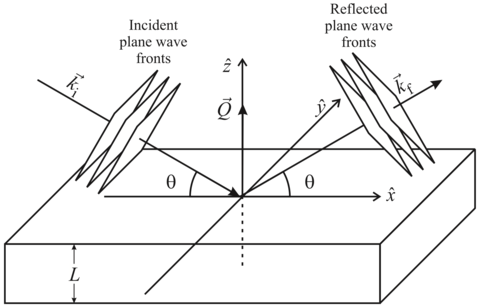
\includegraphics[width=0.7\textwidth]{refl_scheme.png}
    \caption{Отражение от поверхности образца}
\end{figure}

\subsection{Классификация источников излучения для рефлектометрии}
Для более глубокого понимания возможностей метода необходимо рассмотреть особенности взаимодействия различных видов излучения с веществом, что определяет специфику применения рентгеновской и нейтронной рефлектометрии.\\
\begin{figure}[H]
    \centering
    \includegraphics[width=0.7\textwidth]{X-ray_reflectometer.jpg}
    \caption{Принципиальная схема рефлектометра на рентгеновском излучении\\
    X: источник рентгеновского излучения,  
1 и 2: антидисперсионные кристалы монохроматоры,  
3: исследуемый образец,  
D: детектор,  
S: поглотитель излучения. \cite{10}
    }
\end{figure}

\begin{figure}[H]
\centering
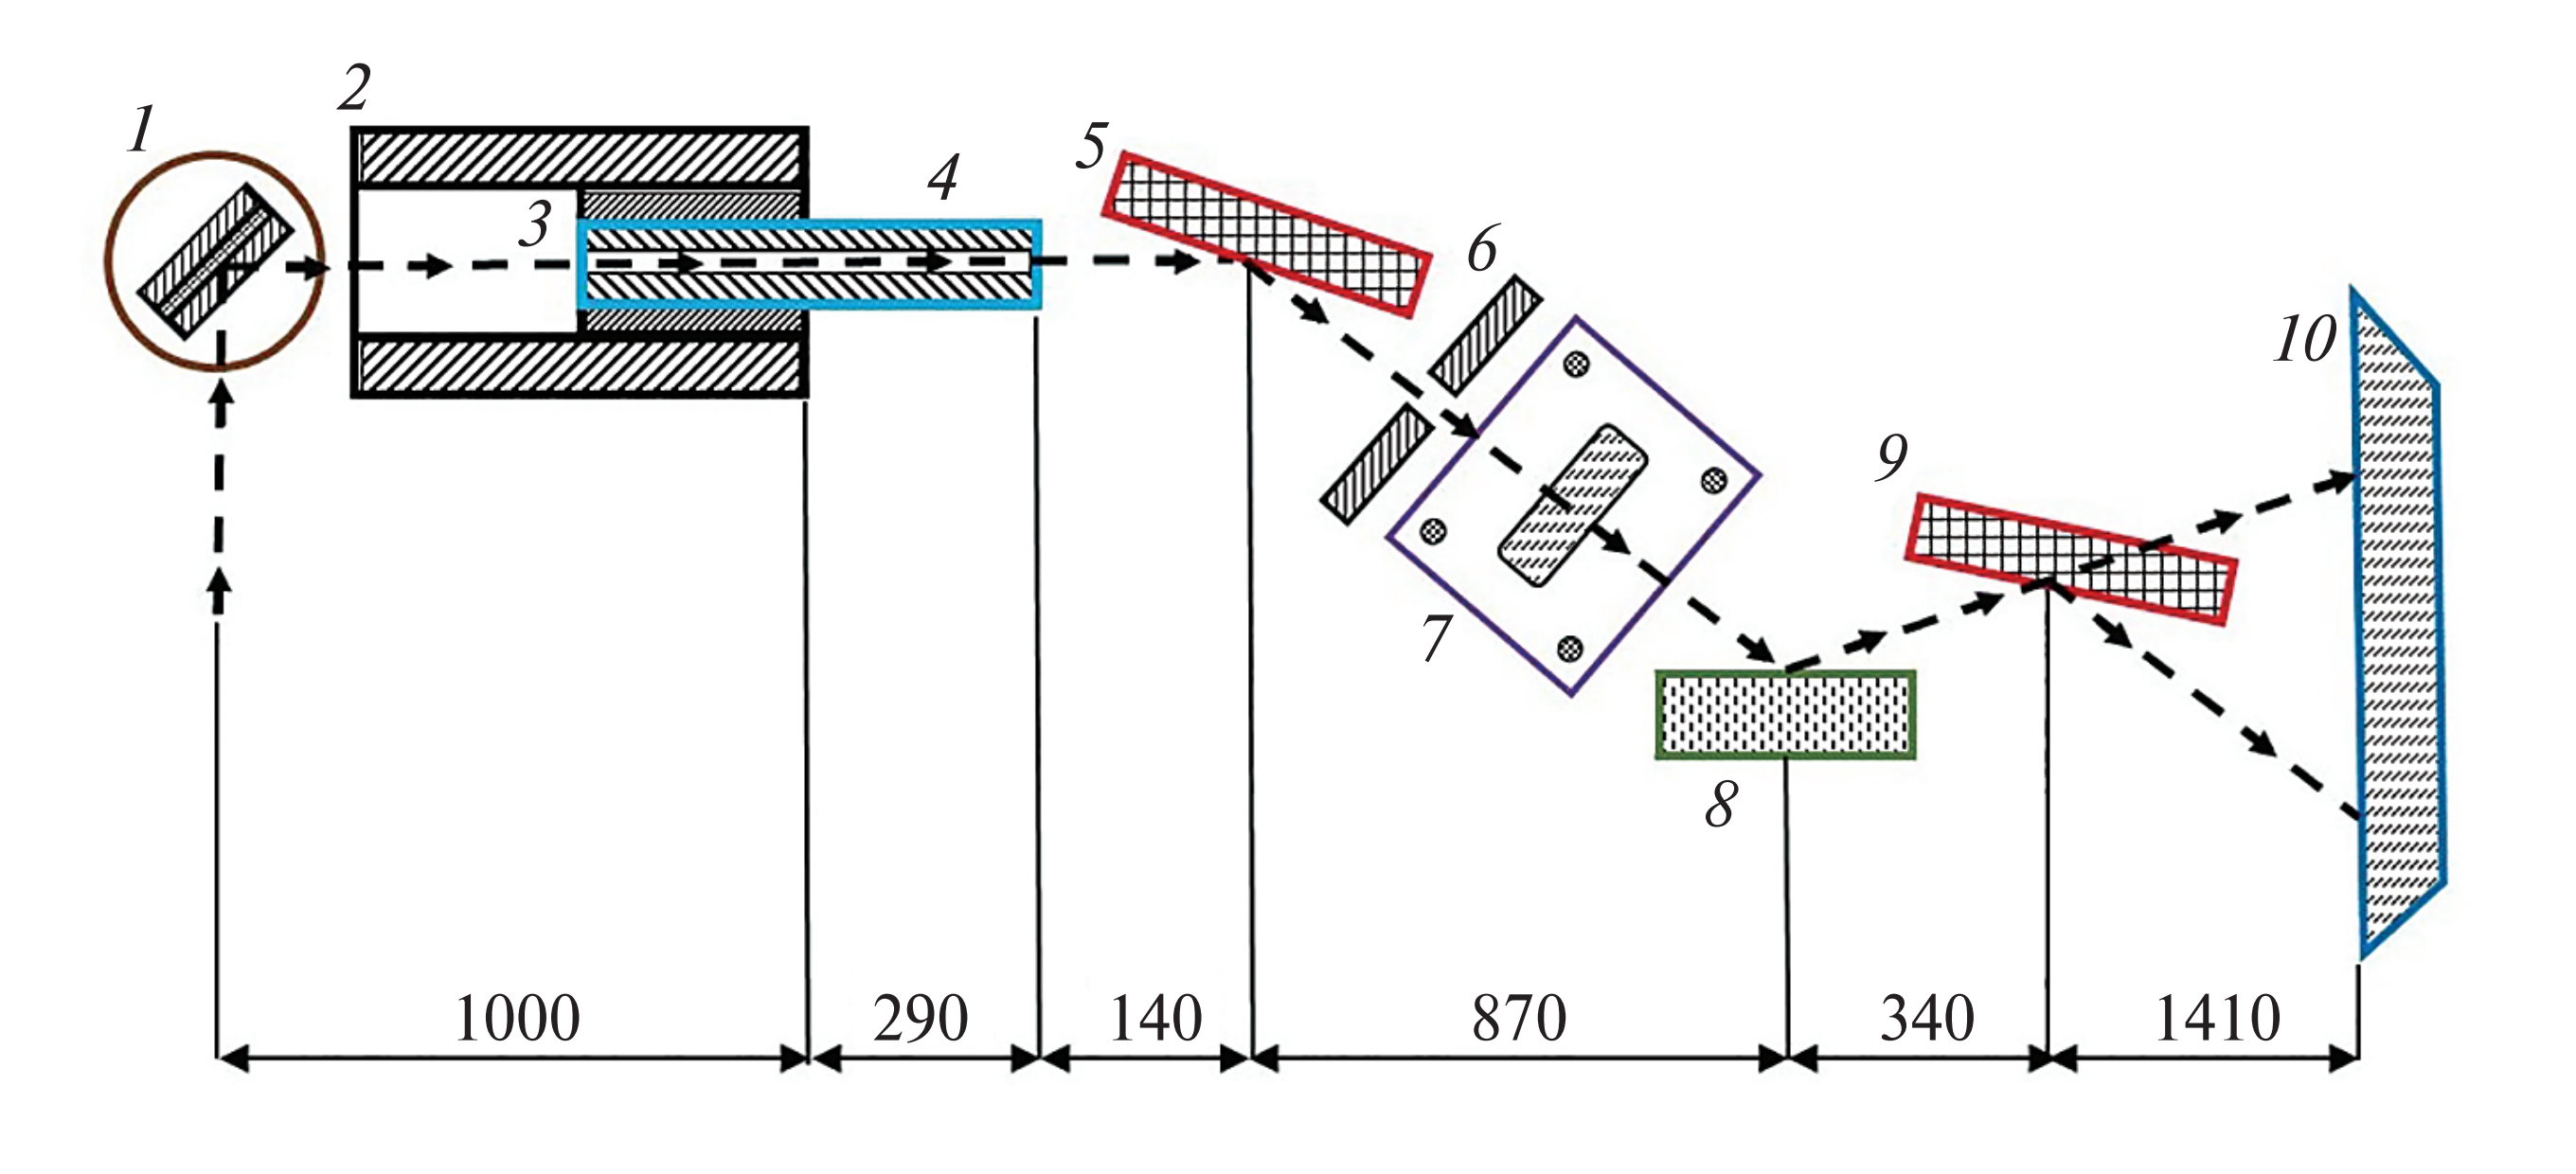
\includegraphics[scale=0.109]{a0000-img001.png}
\caption{Схема стенда нейтронной рефлектометрии на реакторе ИР-8: 1 — монохроматор Cu(111); 2 — канал; 3 — коллиматор ; 4 — вставка в коллиматор; 5 — суперзеркало-поляризатор; 6 — регулируемая щель; 7 — спин-флиппер; 8 — узел образца; 9 — суперзеркало-анализатор; 10 — одномерный позиционно-чувствительный детектор. \cite{14} }
\end{figure}
\subsubsection{Рентгеновская рефлектометрия. Сравнение с нейтронной рефлектометрией}
В рентгеновской рефлектометрии применяются лабораторные источники излучения, такие как герметичные трубки или трубки с вращающимся анодом, а также синхротронные источники и лазеры на свободных электронах, обеспечивающие высокую яркость, регулируемость энергии и возможность временного разрешения. Эти источники обладают значительно более высокой интенсивностью по сравнению с нейтронными, где поток нейтронов обычно составляет 
    $10^6 - 10^8$  \( \frac{\text{нейтронов}}{\text{см}^2 \cdot \text{с}} \)
 в то время как для рентгеновских синхротронных источников светимость может достигать до $10^{12}$
  \( \frac{\text{нейтронов}}{\text{см}^2 \cdot \text{с}} \), что позволяет достигать лучшего отношения сигнала к шуму, проводить измерения с повышенной скоростью и охватывать больший динамический диапазон  \cite{11}. Разрешение рентгеновских рефлектометров выше, чем у нейтронных, прежде всего, благодаря большей интенсивности излучения, облегчающей сбор данных без длительных экспозиций, а также меньшей проникающей способности рентгеновских лучей, которая фокусирует анализ на поверхностных слоях и интерфейсах без значительного рассеяния в объеме образца. Кроме того, более короткие длины волн рентгеновского излучения способствуют лучшей угловой разрешающей способности, минимизируя влияние расходимости пучка.\\
Хотя рентгеновская рефлектометрия обладает преимуществом в виде более высокой интенсивности источника и, как следствие, потенциально большей разрешающей способности, нейтронная рефлектометрия приобретает особую актуальность в тех случаях, когда требуются её уникальные возможности, обусловленные спецификой взаимодействия нейтронов с веществом. Эти преимущества включают:
Во-первых, электрическая нейтральность позволяет нейтронам беспрепятственно преодолевать кулоновский барьер и напрямую взаимодействовать с ядрами атомов. Это обеспечивает значительную глубину проникновения нейтронов в исследуемые материалы — до нескольких сотен нанометров, что существенно превосходит возможности многих поверхностно-чувствительных методов. \\
Во-вторых, длина волны тепловых нейтронов ($\lambda = 0.1-10 $Å)   сопоставима с межатомными расстояниями в конденсированном веществе, что делает их идеальным инструментом для изучения атомной структуры материалов. При этом энергия тепловых нейтронов (5-100 мэВ) сравнима с энергией многих коллективных возбуждений в твердых телах. \\
В-третьих, взаимодействие нейтронов происходит непосредственно с атомными ядрами, а не с электронными оболочками, как в случае рентгеновского излучения. Это приводит к существенно иной зависимости сечения рассеяния от атомного номера элемента. Например, нейтроны весьма чувствительны к лёгким элементам, которые практически "прозрачны" для рентгеновских лучей. Более того, нейтроны способны различать изотопы одного элемента, что открывает широкие возможности для изотопного контрастирования в исследованиях сложных систем.
Наконец, нейтроны обладают собственным магнитным моментом, благодаря чему они чувствительны к магнитной микроструктуре исследуемых образцов. Это свойство позволяет методам нейтронного рассеяния получать уникальную информацию о магнитном упорядочении в веществе, что особенно ценно при изучении магнитных многослойных наноструктур, спиновых волн и магнитных доменов.
\\
Существуют два основных экспериментальных подхода к проведению измерений в нейтронной рефлектометрии, каждый из которых имеет свои преимущества и области применения - угловой и времяпролётный. \\
При использовании углового метода эксперимент проводится с монохроматическим пучком нейтронов с фиксированной длиной волны $\lambda. $ Измерения коэффициента отражения R осуществляются путём последовательного изменения угла падения $\theta $ нейтронного пучка на поверхность образца. Переданный импульс в направлении нормали к поверхности при этом рассчитывается как:

\begin{equation}
 q_z=\frac{4\pi }{\lambda }\sin \theta,
\end{equation}
где $\lambda$ — длина волны нейтронов. \cite{15}\\
Преимущества данного метода включают высокое угловое разрешение и относительную простоту экспериментальной реализации. Угловой метод особенно эффективен на стационарных источниках нейтронов.
Типичный диапазон измерений углов составляет от 0° до 5-10°.\\
Альтернативным подходом является времяпролётная методика, которая особенно эффективна на импульсных источниках нейтронов. В этом случае угол падения $\theta $ фиксируется, а измерения проводятся одновременно для нейтронов различных энергий и, соответственно, длин волн. Распределение нейтронов по энергиям определяется путём измерения времени их пролёта от источника до детектора.
Переданный импульс при этом меняется за счёт вариации длины волны $ \lambda $, где $\lambda$ зависит от времени пролёта t согласно соотношению (7).
Ключевые преимущества времяпролётного метода:
одновременное измерение в широком диапазоне $q_z$, 
отсутствие подвижных частей во время измерения,
высокая эффективность использования нейтронного пучка,
возможность работы с малыми образцами или слабыми сигналами.
Современные времяпролётные рефлектометры часто оснащаются позиционно-чувствительными детекторами, что позволяет одновременно регистрировать как зеркально отражённые нейтроны, так и диффузное рассеяние, несущее информацию о латеральных неоднородностях и шероховатости поверхности.\\
Ключевым элементом любой нейтронной рефлектометрической установки выступает источник нейтронов, который определяет как возможности, так и ограничения данного метода.

Нейтронные источники классифицируются на два основных типа: стационарные и импульсные. Принципиальное различие между ними заключается в характере генерации нейтронного потока, что непосредственно влияет на конструкцию рефлектометров и применяемые методы монохроматизации. Эти особенности, в свою очередь, определяют параметры нейтронных потоков, что впоследствии оказывает существенное влияние на специфику и возможности проводимых экспериментов.

\subsubsection{Стационарные источники нейтронов}
Стационарные источники, представленные преимущественно исследовательскими ядерными реакторами (ИР-8, ПИК, ИВВ-2М), производят непрерывный поток нейтронов с широким энергетическим спектром. Первичный спектр тепловых нейтронов описывается максвелловским распределением:

\begin{equation}
A(\lambda) \sim \lambda^{-5} \exp\left(-\frac{h^2}{2mk T\lambda^2}\right)
\end{equation}

где $h$ -- постоянная Планка, $m$ -- масса нейтрона, $k$ -- постоянная Больцмана, $T$ -- температура замедлителя \cite{15}.

При термализации нейтронов в активной зоне реактора максимум спектральной плотности приходится на длину волны $\lambda_{max} = \sqrt{\frac{5h^2}{2mkT}}$. Для реактора с температурой замедлителя $T = 300$ К оптимальная длина волны составляет около 1.45 \AA, что соответствует энергии нейтронов примерно 39 мэВ.

На стационарных источниках монохроматизация нейтронного пучка осуществляется с помощью кристаллических монохроматоров, использующих брэгговское отражение:

\begin{equation}
\lambda = 2d \cdot \sin(\theta_M)
\end{equation}

где $d$ -- межплоскостное расстояние в кристалле, $\theta_M$ -- угол скольжения.

Пучок, отраженный от монохроматора, имеет расходимость, 
которая определяется сверткой расходимости падающего пучка $\Delta\theta_{in}$ и мозаичности кристалла $\eta$ \cite{15}:

\begin{equation}
\frac{1}{(\Delta\theta_{out})^2} = \frac{1}{(\Delta\theta_{in})^2} + \frac{1}{\eta^2}
\end{equation}

При этом относительная монохроматичность пучка связана с расходимостью соотношением \cite{15}:

\begin{equation}
\frac{\Delta\lambda}{\lambda} = \Delta\theta \cdot \cot(\theta_M)
\end{equation}

В данном случае аппаратная функция рефлектометра характеризуется разрешением по переданному импульсу \cite{15}:

\begin{equation}
\frac{\Delta q}{q} = \sqrt{\left(\frac{\Delta\theta}{\theta}\right)^2 + \left(\frac{\Delta\lambda}{\lambda}\right)^2}
\end{equation}

Оптимизация светосилы рефлектометра на стационарном источнике достигается при соотношении \cite{15}:

\begin{equation}
\frac{\Delta\theta}{\theta} = \frac{1}{2} \cdot \frac{\Delta q}{q}
\end{equation}

что позволяет максимизировать интенсивность при заданном разрешении.

\subsubsection{Импульсные источники нейтронов}
Импульсные источники включают:
\begin{itemize}
    \item Ускорители с мишенями (ISIS, SNS, ESS), использующие реакции скалывания при бомбардировке тяжелых мишеней высокоэнергетическими частицами 
    \item Импульсные реакторы (ИБР-2) 
    \item Лазерные нейтронные источники, основанные на DD- или DT-реакциях синтеза 
\end{itemize}

В таких системах нейтроны генерируются короткими импульсами, что позволяет применять времяпролетный метод (TOF) для определения длины волны нейтронов:

\begin{equation}
\lambda = \frac{h \cdot t}{m \cdot L}
\end{equation}

где $t$ -- время пролета, $L$ -- расстояние от источника до детектора.

Времяпролетная методика позволяет измерять кривые отражения в широком диапазоне длин волн за один импульс источника, что существенно увеличивает эффективность использования нейтронного потока. Основное разрешение в этом случае определяется временным разрешением:

\begin{equation}
\frac{\Delta\lambda}{\lambda} = \frac{\Delta t}{t}
\end{equation}

В зависимости от типа прерывателя (чоппера) в системе, аппаратная функция может быть разной:
\begin{enumerate}
    \item Однодисковый прерыватель обеспечивает постоянное времяпролетное разрешение $\Delta t$, поэтому $\Delta\lambda = \text{const}$, что приводит к $\frac{\Delta\lambda}{\lambda} \sim \frac{1}{\lambda}$. 
    \item Двухдисковый прерыватель позволяет получить $\frac{\Delta\lambda}{\lambda} = \text{const}$ во всем диапазоне длин волн. 
\end{enumerate}

При времяпролетной методике разрешение по переданному импульсу выражается как \cite{15}:

\begin{equation}
\frac{\Delta q}{q} = \sqrt{\left(\frac{\Delta\theta}{\theta}\right)^2 + \left(\frac{\Delta t}{t}\right)^2}
\end{equation}

Оптимизация светосилы рефлектометра на импульсном источнике достигается при условии:

\begin{equation}
\frac{\Delta\theta}{\theta} = \frac{1}{\sqrt{2}} \cdot \frac{\Delta t}{t}
\end{equation}

\subsection*{Создание нейтронных пучков для нейтронной рефлектометрии}

Для задач нейтронной рефлектометрии необходимо создать поток нейтронов с определённой энергией, поляризацией и направлением движения.

Стационарные источники нейтронов характеризуются постоянным нейтронным потоком от контролируемой реакции ядерного деления в ядерном реакторе, могут базироваться на следующих реакциях:

\begin{itemize}
    \item Спонтанное деление ядер:
    \begin{align*}
        ^{252}\text{Cf} &\to \text{осколки деления} + \sim3.77\,\text{нейтрона/деление} + \sim\SI{200}{MeV} \\
        ^{240}\text{Pu} &\to \text{осколки деления} + \sim2.2\,\text{нейтрона/деление} + \sim\SI{200}{MeV}
    \end{align*}
    
    \item Радионуклидные ($\alpha$,n)-источники --- комбинация $\alpha$-излучателя (например, \(^{241}\text{Am}\), \(^{226}\text{Ra}\), \(^{210}\text{Po}\)) и мишени из легкого элемента (обычно Be, Li или B), при взаимодействии происходит реакция вида:
    \[
    \alpha + {}^9\text{Be} \to {}^{12}\text{C} + n
    \]
    
    \item Фотонейтронные источники --- $\gamma$-излучение взаимодействует с ядрами определенных элементов:
    \begin{align*}
        ^9\text{Be} + \gamma &\to {}^8\text{Be} + n + \SI{1.67}{MeV} \\
        ^2\text{H} + \gamma &\to {}^1\text{H} + n + \SI{2.22}{MeV}
    \end{align*}
    
    \item Ядерные реакторы --- поддерживаемая цепная реакция деления тяжелых ядер:
    \begin{align*}
        ^{235}\text{U} + n &\to \text{осколки деления} + \sim2.43\,\text{нейтрона/деление} + \sim\SI{200}{MeV} \\
        ^{239}\text{Pu} + n &\to \text{осколки деления} + \sim2.87\,\text{нейтрона/деление} + \sim\SI{200}{MeV}
    \end{align*}
\end{itemize}

Импульсные источники могут базироваться на:

\begin{itemize}
    \item Механическом прерывателе (чоппере) со стационарным источником. Непрерывный поток нейтронов прерывается вращающимся механическим устройством, поток «нарезается» на короткие импульсы с частотой вращения прерывателя.
    
    \item Ускоритель заряженных частиц в импульсном режиме с мишенью.
    
    \item Импульсные реакторы. Механизм генерации импульса:
    \begin{itemize}
        \item Реактор сначала приводится в подкритическое состояние,
        \item затем быстро вводится положительная реактивность (например, перемещением отражателя, извлечением поглотителя или специальными импульсными стержнями),
        \item мощность реактора начинает экспоненциально расти,
        \item рост прекращается за счет отрицательной обратной связи (тепловое расширение топлива, доплеровский эффект),
        \item после пика мощность быстро падает.
    \end{itemize}
    
    \item Создание условий для термоядерного синтеза:
    \begin{align*}
        ^2\text{H} + {}^3\text{H} &\to {}^4\text{He} + n + \SI{17.6}{MeV} \\
        ^2\text{H} + {}^2\text{H} &\to {}^3\text{He} + n + \SI{3.27}{MeV}
    \end{align*}
    Лазерный синтез: мощные лазерные импульсы сжимают мишень; \\
    Z-пинч устройства: сверхвысокий ток создает мощное магнитное поле.
\end{itemize}

\subsection*{Влияние температуры источника}
Нейтронная рефлектометрия применяется для изучения твёрдых тел с характерным межатомарным расстоянием в кристаллической решётке около \SI{1}{\angstrom}. Для исследования таких структур требуется излучение с соответствующей длиной волны. Для нейтронов такая длина волны достигается при энергиях порядка 0.01 эВ, что соответствует холодным нейтронам. Однако первичный спектр нейтронов от ядерного реактора довольно широк, максимум спектральной плотности приходится на энергии порядка 2 МэВ, что явно не подходит для задач нейтронной рефлектометрии. Это энергетическое несоответствие требует создания специализированных систем для замедления нейтронов до требуемого энергетического диапазона.\\
Так, cущественным фактором является температура нейтронного источника. Для тепловых источников ($T \approx 300$ К) максимум спектра приходится на $\lambda \approx 1.12$ \AA, для холодных ($T \approx 30$ К) -- на $\lambda \approx 3.56$ \AA. При прочих равных условиях, переход к холодному источнику увеличивает светосилу рефлектометра пропорционально $\sqrt{\frac{T_1}{T_2}}$, что для указанных температур дает прирост примерно в 3.16 раза.

Холодные нейтроны также обеспечивают лучшее $q$-разрешение, поскольку при той же коллимации пучка $\Delta\theta$ относительная монохроматичность $\frac{\Delta\lambda}{\lambda}$ улучшается с ростом длины волны $\lambda$. Кроме того, эффективность транспортировки нейтронов от источника к образцу выше для холодных нейтронов из-за более эффективного захвата и удержания их в нейтроноводах. \cite{15}

Таким образом, выбор типа нейтронного источника и его характеристик определяет подход к монохроматизации нейтронного пучка, конструкцию рефлектометра и, в конечном счете, аппаратную функцию прибора, что напрямую влияет на возможности и ограничения экспериментальных исследований.

\subsubsection*{Процесс замедления нейтронов}

Замедление нейтронов из реакторных источников включает несколько этапов:

\begin{enumerate}
    \item Начальное замедление с помощью бериллия непосредственно в активной зоне реактора    
    \item Последующее замедление с использованием водных замедлителей (как H\textsubscript{2}O, так и D\textsubscript{2}O) для снижения энергии нейтронов до уровня, требуемого для экспериментов по рефлектометрии     
    \item Транспортировка по нейтроноводам, которые также смещают пик энергетического спектра в область более низких энергий \end{enumerate}

\begin{figure}[H]
    \centering
    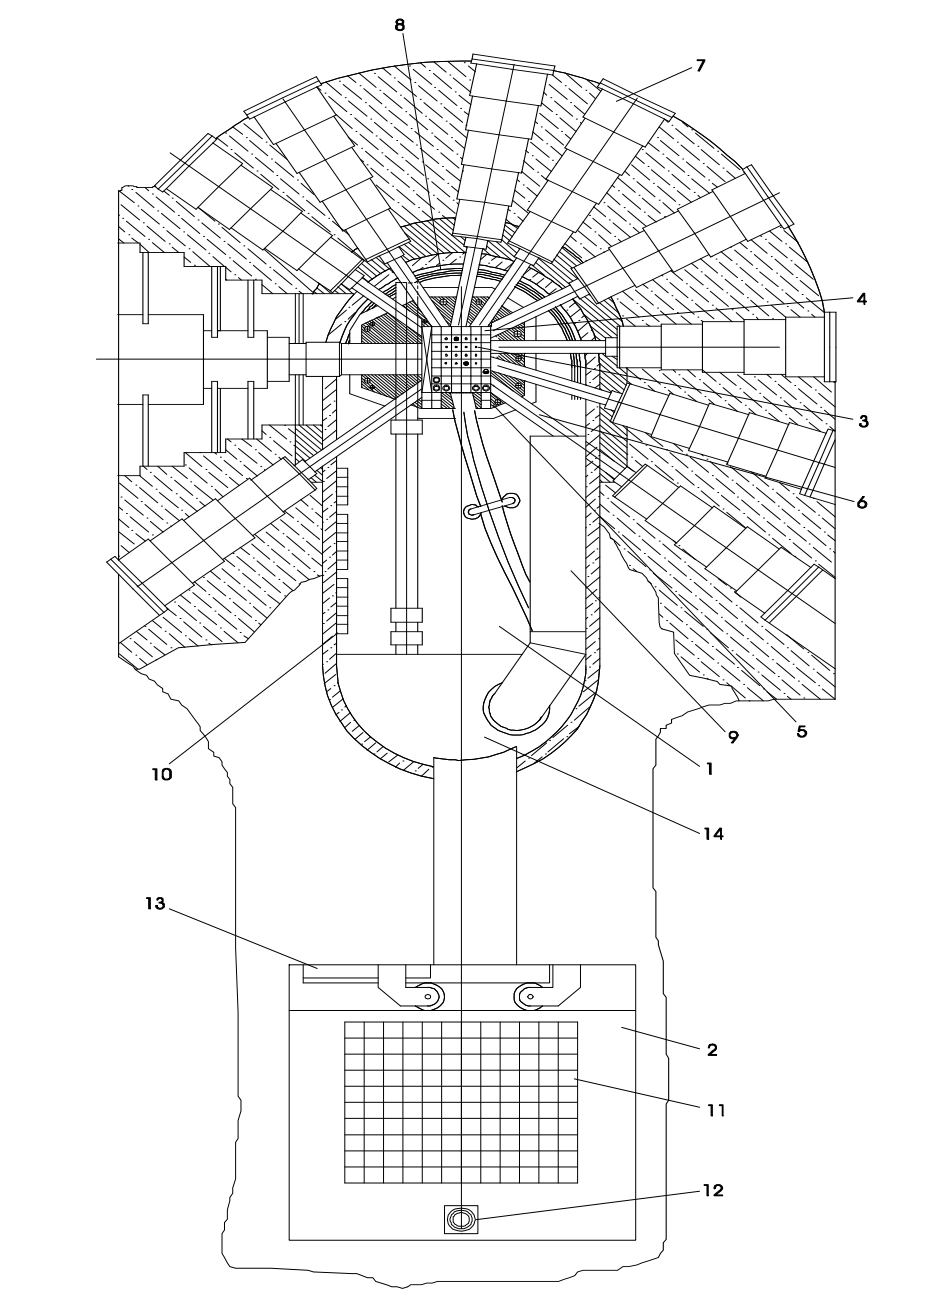
\includegraphics[width=0.6\textwidth]{разрез_ир8.png}
    \caption{Поперечный разрез реактора ИР-8: 
        1 – бассейн реактора; 
        2 – бассейн хранилища; 
        3 – ТВС; 
        4 – сменный бериллиевый блок; 
        5 – стационарный бериллиевый блок; 
        6 – Горизонтальный экспериментальный канал; 
        7 – шибер; 
        8 – стальной экран; 
        9 – задерживающая емкость; 
        10 – временное хранилище ОТВС; 
        11 – хранилище ОТВС; 
        12 – ведро контейнера для выгрузки ТВС из бассейна; 
        13 – ворота шлюза; 
        14 – крышка распределительного короба}
    \label{fig:ir8-cutaway}
\end{figure}

\subsubsection*{Транспортировка холодных нейтронов}

Холодные нейтроны доставляются к рефлектометрам по нейтроноводам. Эти нейтроноводы спроектированы с определенными оптическими свойствами для эффективной транспортировки нейтронов с сохранением желаемых характеристик пучка.

Типы нейтроноводов:

\begin{enumerate}
    \item Прямые --- базовая транспортировка с постоянным сечением    
    \item Изогнутые --- устраняют прямую видимость источника, снижая фон излучения    
    \item Баллистические --- с расширяющимися/сужающимися секциями для минимизации потерь    
    \item Переменного сечения (эллиптические, параболические) --- оптимизируют характеристики пучка    
    \item Фокусирующие --- концентрируют пучки для увеличения плотности потока \end{enumerate}

Материалы:

\begin{itemize}
    \item Никель --- высокие критические углы    
    \item Суперзеркальные покрытия (многослойные Ni/Ti)
    \item Подложки: борированное стекло, кремний, алюминий\end{itemize}

Суперзеркала характеризуются $m$-значением --- отношением критического угла к углу природного никеля, что значительно повышает эффективность транспортировки.

\bigskip

Так, например, исследовательский ядерный реактор бассейнового типа ИР-8 (рис. 1, 2) предназначен для проведения фундаментальных и прикладных исследований в различных областях науки и техники: в области ядерной физики, физики твёрдого тела и сверхпроводимости, нанотехнологий и наноматериалов, радиационного материаловедения, нейтронно-активационного анализа элементного состава вещества, испытаний образцов новых топливных композиций для перспективных энергетических реакторных установок, наработки изотопов медицинского назначения. Активная зона реактора расположена под десятиметровым слоем дистиллированной воды, а в активной зоне используются бериллиевые блоки. На реакторе имеется 12 горизонтальных каналов, из которых:

\begin{itemize}
    \item 9 радиальных ГЭК с внутренним диаметром 100 мм;
    
    \item 1 касательный сквозной ГЭК с внутренним диаметром 150 мм;
    
    \item 1 специальный ГЭК с внутренним диаметром 230 мм, используемый для размещения в нем источника холодных нейтронов;
    
    \item 1 криволинейный ГЭК для вывода ультрахолодных нейтронов.
\end{itemize}

В настоящее время на ГЭК № 10 экспериментальные устройства и оборудование демонтированы. На этом канале сооружается источник холодных нейтронов с комплексом нейтроноводов и экспериментальных установок. Источник холодных нейтронов предназначен для формирования интенсивного потока нейтронов с длиной волны \(\sim\SI{4}{\angstrom}\).

Для проведения исследований на горизонтальных каналах реактора ИР-8 имеется комплекс нейтронно-физической аппаратуры, в состав которого входят различные исследовательские инструменты, в том числе:

\begin{itemize}
    \item Нейтронный рефрактометр;
    
    \item Трёхосный кристаллический спектрометр;
    
    \item Поликристалльный многодетекторный кольцевой дифрактометр;
    
    \item Трёхосный спектрометр на идеальных кристаллах.
\end{itemize}

\begin{figure}[h]
    \centering
    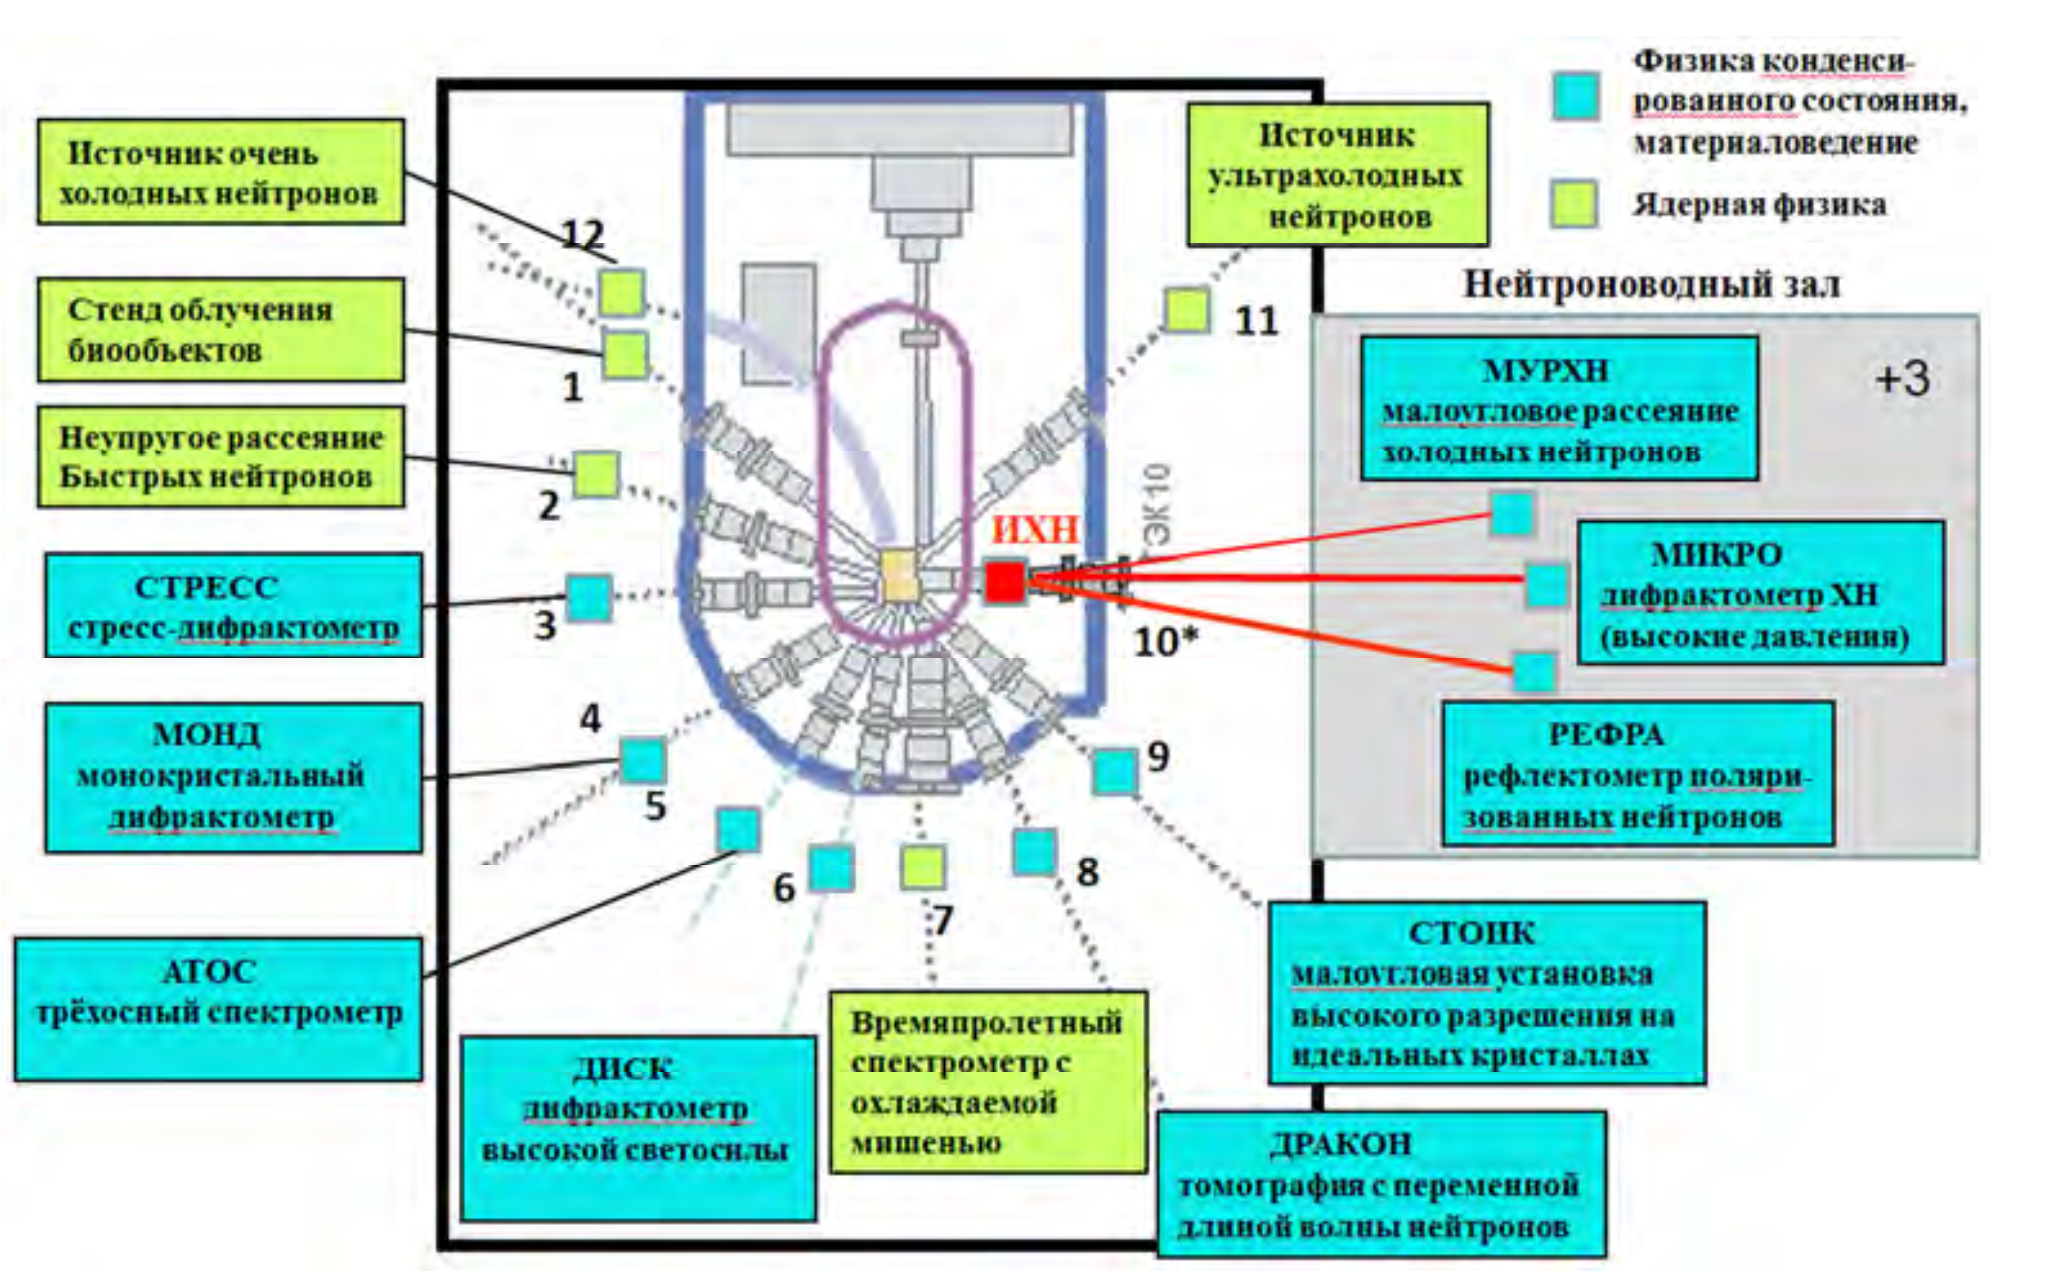
\includegraphics[width=0.8\textwidth]{ир8.png}
    \caption{ Курчатовский нейтронный центр на базе реактора ИР-8}
\end{figure}

Планируется установить три нейтроновода, 
на выходе которых интегральный поток нейтронов будет 
\(2 \times 10^{8}\,\text{\textit{см}}^{-2}\text{\textit{с}}^{-1}\) 
с максимумом спектра вблизи длины волны нейтронов \(4{,}5\,\text{\AA}\). 
На нейтроноводах будут установлены три установки: 
спектрометр малоуглового рассеяния холодных нейтронов (МУРХН), 
дифрактометр для исследования микрообразцов под высоким давлением (МИКРО) 
и рефлектометр поляризованных нейтронов (РЕФРА).
%\cite{ковальчук2017развитие}



\subsection*{Теория и методы}

\subsection{Метод Абелевых матриц}
Для интерпретации экспериментальных данных рефлектометрии и моделирования поведения зондирующего излучения в многослойных структурах используется метод Абелевых матриц. Этот метод позволяет решить прямую задачу рефлектометрии, заключающуюся в расчете зависимости комплексного коэффициента отражения от нормальной компоненты переданного импульса по заданной структуре образца.\\
Метод Абелевых матриц базируется на решении классической задачи квантовой механики о прохождении волной потенциального барьера, где, в данном случае, в роли волны выступают нейтроны или рентген, а в роли потенциального барьера  - образец. Математически, задача сводится к решению стационарного уравнения Шрёдингера:
\begin{align}
    \Bigg(\frac{\hbar^2}{2m_n}\nabla^2 + U(\vec{r})\Bigg)\Psi(\vec{r}) = E\Psi(\vec{r})
\end{align}
где $m_n$ - масса нейтрона, $U(r)$ - потенциальная энергия. \cite{9, 13}

Заменив \begin{align}
\Psi(\vec{r}) = \psi(y)e^{{i} k_{||} q_{||}}
\end{align}
где $k_{\parallel}$ - волновой вектор, параллельный поверхности образца,

и $\psi(y)$ соответствует одномерному уравнению Шрёдингера \cite{13}:
\begin{equation}
    \left( \frac{d^2}{dy^2} + \left( \frac{2m_n}{\hbar^2}(E - U) - k_{\parallel}^2 \right) \right) \psi(y) = 0
\end{equation}

Следовательно, для $\alpha$-го слоя имеем:
\begin{equation}
    \Bigg( \frac{d^2}{dy^2} + q_{\alpha}^2 \Bigg) \psi(y) = 0
\end{equation}
где \begin{equation}
    q_{\alpha} = \Bigg(\frac{2m_n}{\hbar^2}(E - \frac{\hbar^2 k_{\parallel}^2}{2m_n} - U_{\alpha})\Bigg)^{1/2}
\end{equation}

Теперь можем записать волновую функцию в слое \alpha $как суперпозицию волн, 
распространяющихся по оси y и против оси y \cite{9}: 

\begin{equation}
    \psi_{\alpha}(y) = a_{\alpha}e^{iq_{\alpha}(y- y_{\alpha})} + b_{\alpha}e^{-iq_{\alpha}(y- y_{\alpha})}
\end{equation}

Представим \psi_{\alpha}(y)|_{y = y_{\alpha}} $вектором \(
\begin{bmatrix}
a_{\alpha}\\
b_{\alpha}
\end{bmatrix}
\).

\text{Так, первой поверхности будет соответствовать:}
\psi_1 |_{y_1 = 0} = \(
\begin{bmatrix}
1\\
r
\end{bmatrix}
\) 

\text{Последней поверхности: } \psi_{n-1} |_{y_{n-1}} = \(
\begin{bmatrix}
t\\
0
\end{bmatrix} 
\) 

Следовательно, коэффициенты поглощения t и отражения r могут быть определены матрицой передачи:
\begin{equation}
     \(
\begin{bmatrix}
1\\
r
\end{bmatrix}
\)  = \(
\begin{bmatrix}
M_{11} & M_{12}\\
M_{21} & M_{22}
\end{bmatrix}
\) \(
\begin{bmatrix}
t\\
0
\end{bmatrix} 
\),
\end{equation}
 коэффициенты r и t могут быть выражены: 
\begin{equation}
    t = \frac{1}{M_{11}},  r = \frac{M_{21}}{M_{22}}
\end{equation}

Матрица передачи M выражается следующим образом \cite{9} :
\begin{equation}
    M = D^{-1}(q_1)\Bigg(\prod\limits_{j=2}^{N-1}[D(q_j)P(d_j , q_j)D^{-1}(q_j)]\Bigg)D(q_N),
\end{equation} \text{где} D(q_{\alpha}) - \text{матрица передачи, отвечающая за изменение абсолютного значения} \\
\text{волнового вектора в среде }  \alpha;

P(d_{\alpha} , q_{\alpha}) - \text{матрица распространения, отвечающая за изменение фазы волнового вектора}\\
\text{в среде } \alpha.

\begin{equation}
    D(q_{\alpha}) = \(
\begin{bmatrix}
1 & 1\\
q_{\alpha} & -q_{\alpha}
\end{bmatrix}
\)
\end{equation}

\begin{equation}
    P(q_{\alpha}, d_{\alpha}) = \(
\begin{bmatrix}
e^{-iq_{\alpha}d_{\alpha}} & 0\\
0 & e^{iq_{\alpha}d_{\alpha}}
\end{bmatrix}
\)
\end{equation}

\subsection{Свёртка. Аппаратная функция}

Свёртка – операция, применяющаяся к двум функциям, возвращающая их взаимнокорреляционную функцию. Так, применяя оператор свёртки для истинного распределения и аппаратной функции, получим измеренное распределение физической величины. 

\begin{figure}[h]
    \centering
    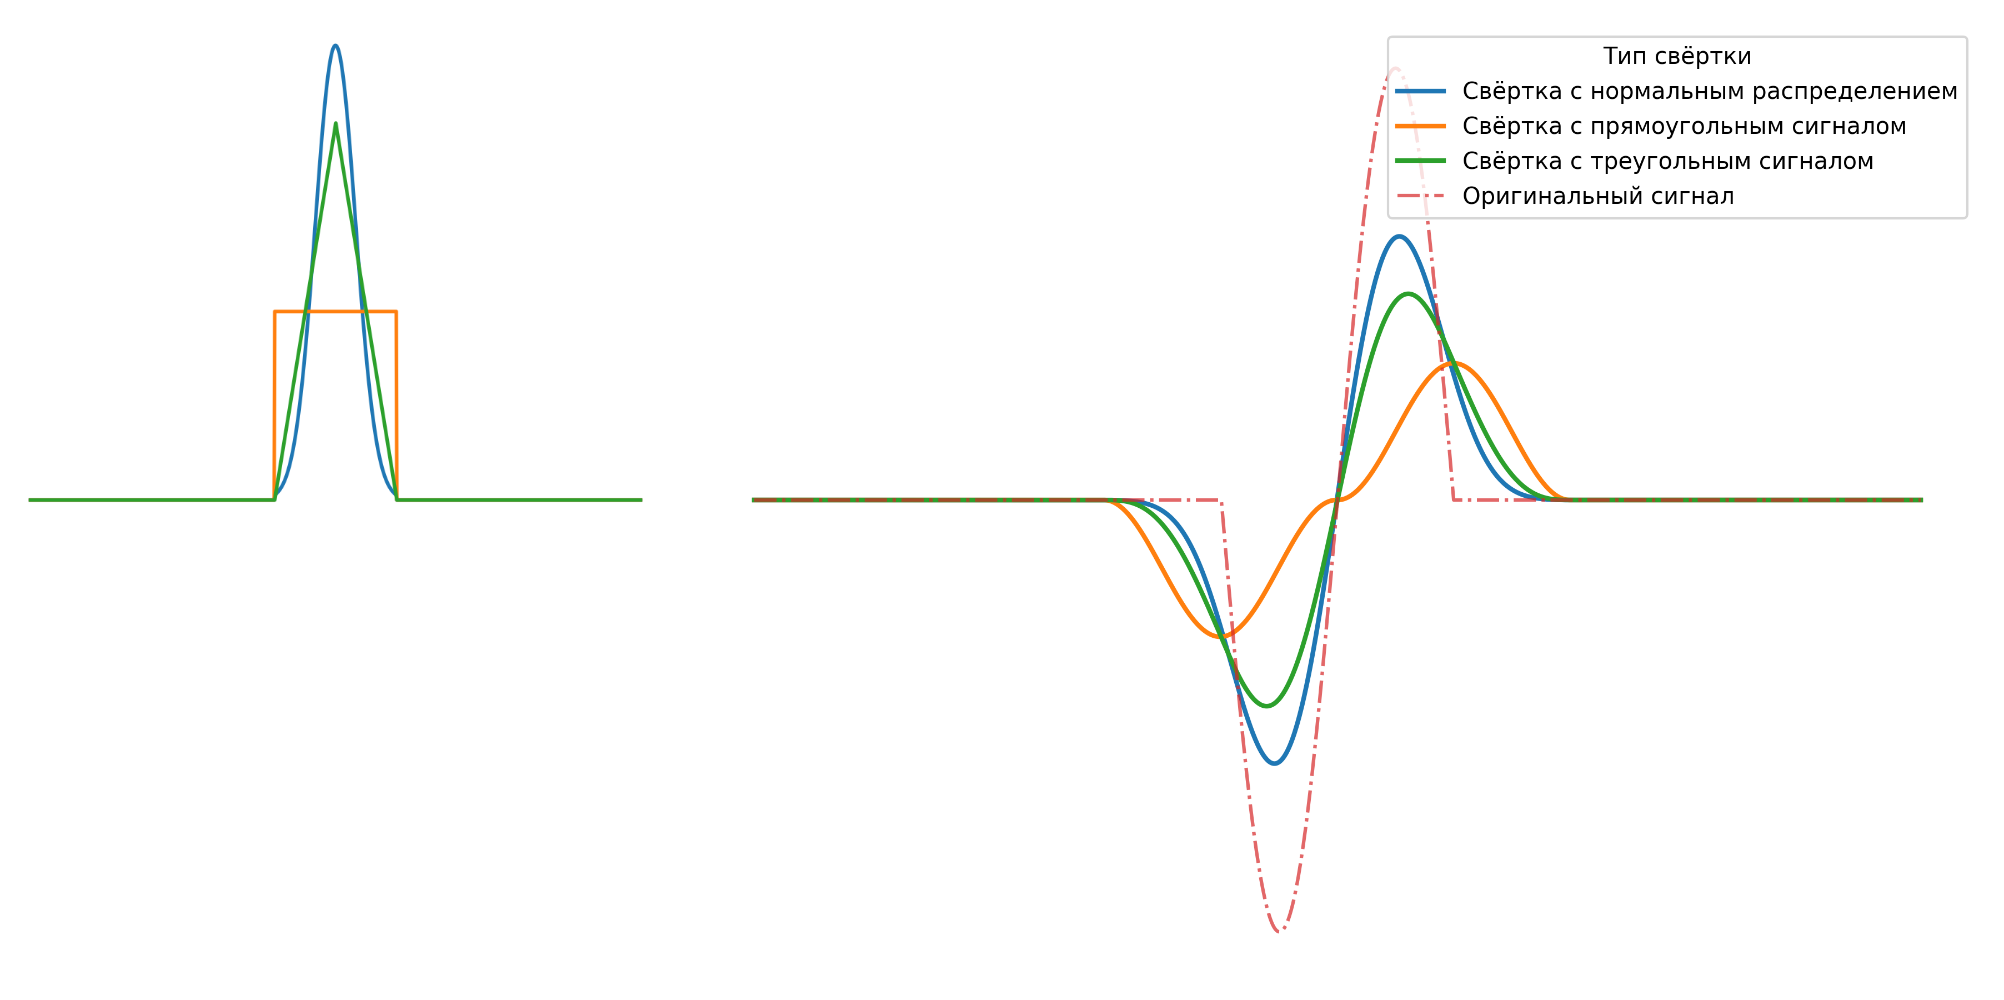
\includegraphics[width=0.7\textwidth]{conv_h.png}
    \caption{Иллюстрация работы свёртки}
\end{figure}

Свёртка играет важную роль в моделировании искажений, связанных с ограниченным разрешением измерительных устройств.
Поскольку приборы не способны идеально воспроизводить входной сигнал (например, из-за физических ограничений оптики или электроники), их влияние на измеряемую величину можно описать как свёртку истинного распределения $\varphi
\left(x\right)$ с аппаратной функцией $a\left(x\right)$. Это позволяет теоретически предсказать, как будут выглядеть экспериментальные данные при заданных параметрах установки.

На практике задача восстановления исходного распределения $\varphi \left(x\right)$ из измеренного сигнала 
$f\left(x\right)$ (т.н. обратная свёртка) является сложной и решается лишь в специальных случаях, например, при определённых условиях гладкости функций или наличии априорной информации о системе. Наиболее часто свёртка используется для симуляции ожидаемых искажений. Например, при проектировании спектрометров или радиотелескопов с её помощью моделируют ``размытие'' спектральных линий или изображений, что помогает оценить пределы разрешающей способности прибора и скорректировать экспериментальные параметры.

\textbf{Теорема о свёртке.}

Если $h(x) = (f \ast g)(x)$ --- свёртка функций $f(x)$ и $g(x)$, то их преобразование Фурье удовлетворяют соотношению:

\begin{equation}
\mathcal{F}\{h\}(k) = \mathcal{F}\{f\}(k) \cdot \mathcal{F}\{g\}(k)
\end{equation}

где:
\begin{itemize}
\item $\mathcal{F}\{f\}(k) = \int_{-\infty}^{+\infty} f(x)e^{-ikx}dx$ --- преобразование Фурье функции $f(x)$
\item $\mathcal{F}\{g\}(k)$ --- преобразование Фурье функции $g(x)$
\end{itemize}

\textbf{Обратное преобразование.}

Свёртка в исходном пространстве восстанавливается через обратное преобразование Фурье:

\begin{equation}
h(x) = \mathcal{F}^{-1}\{\mathcal{F}\{f\} \cdot \mathcal{F}\{g\}\}
\end{equation}

В исследованиях возникают как задачи, связанные с вычислением истинного распределения $\varphi \left(x\right)$, так и задачи, связанные с моделированием измеренного распределения $f\left(x\right)$ физической величины с учётом параметров установки.

Задача нахождения $\varphi \left(x\right)$ сводится к решению интегрального уравнения (1) с помощью преобразования Фурье, при этом решение может быть выполнено только для некоторых видов функций $f\left(x\right)$ и 
$a\left(x\right)$.

\textbf{Аппаратная функция.}

Аппаратная функция --- характеристика линейного измерительного устройства, устанавливающая связь измеренной величины на выходе устройства с истинным значением этой величины на его входе. Математически аппаратная функция определяется из уравнения 
\begin{equation}
f(x) = \int_{-\infty}^{+\infty} a(x-x_1)\varphi(x_1)dx_1
\end{equation}

где $f(x)$ --- измеренное распределение физической величины, $\varphi(x)$ --- истинное распределение, $a(x)$ --- аппаратная функция.

Аппаратная функция может быть рассчитана теоретически по известным параметрам измерительного устройства, однако это представляет собой достаточно сложную задачу и даёт, как правило, приближённые результаты. Поэтому очень часто аппаратную функцию определяют экспериментальным путём. Так, аппаратная функция оптического спектрометра может быть измерена с достаточно большой точностью, если для освещения входной щели использовать излучение с выхода другого спектрометра с известной аппаратной функцией, на 1-2 порядка меньшей ширины, чем у данного, либо использовать источник с узкой спектральной линией, в окрестностях которой перестраивается (по длинам волн, частотам или обратным сантиметрам)
спектрометр с измеряемой аппаратной функцией. При таком измерении форма и ширина аппаратной функции будут определены точнее, чем расчётным путём, так как при этом учитываются даже неточности юстировки, которые никак не могут быть учтены при расчёте. Рассчитанная или измеренная аппаратная функция реальных приборов на практике аппроксимируется с помощью ряда функций.

Так, аппаратная функция является не только и не столько критерием разрешения, сколько характеристикой прибора, знание которой позволяет вычислить истинное распределение в спектре величины, характеризующей изучаемое явление. 

\subsection{Градиентные методы оптимизации}
Градиентные методы оптимизации представляют собой класс итеративных алгоритмов, предназначенных для нахождения локальных экстремумов  дифференцируемых функций многих переменных. Основная задача, которую они решают, формулируется как минимизация целевой функции $f(\mathbf{x})$ на некотором множестве $\mathcal{K} \subseteq \mathbb{R}^n$, то есть поиск точки $\mathbf{x}^* \in \mathcal{K}$, где значение функции минимально: 
\[
f(\mathbf{x}^*) \leq f(\mathbf{x}) \; \forall \, \mathbf{x} \in \mathcal{K}.
\]
Эти методы используют информацию о градиенте функции $\nabla f(\mathbf{x})$, который указывает направление наибольшего роста, для построения последовательности приближений, начиная с начальной точки и корректируя её в направлении антиградиента для минимизации. Исследования показывают, что такие подходы особенно эффективны для гладких и выпуклых функций, хотя на практике применяются шире, с учётом возможных шумов или ограничений.\\
 \subsubsection{Градиентный спуск}\\
 Подставим в формулу Тейлора $\|\mathbf{h}\| = 1$:

\[
f(\mathbf{x} + \alpha \mathbf{h}) = f(\mathbf{x}) + \alpha \langle \nabla f(\mathbf{x}), \mathbf{h} \rangle + o(\alpha).
\]

Мы хотим уменьшить значение функции, то есть 
\[
f(\mathbf{x}) + \alpha \langle \nabla f(\mathbf{x}), \mathbf{h} \rangle + o(\alpha) < f(\mathbf{x}).
\]

При $\alpha \to 0$ $\langle \nabla f(\mathbf{x}), \Delta \mathbf{x} \rangle \le 0$ при $\alpha \to 0$.  
По неравенству Коши–Буняковского:

\[
\langle \nabla f(\mathbf{x}), \mathbf{h} \rangle \ge -\|\nabla f(\mathbf{x})\|_2 \, \|\mathbf{h}\|_2 = -\|\nabla f(\mathbf{x})\|_2.
\]

Равенство в неравенстве Коши–Буняковского достигается при пропорциональности аргументов, а именно:

\[
\mathbf{h} = -\frac{\nabla f(\mathbf{x})}{\|\nabla f(\mathbf{x})\|_2}.
\]

Рассмотрим точку $\mathbf{x}_0$ в пространстве параметров $\mathcal{K} \subseteq \mathbb{R}^n$ функции $f(\mathbf{x})$.  
Тогда каждую следующую точку выбираем следующим образом:

\begin{equation}
    \mathbf{x}_{k+1} = \mathbf{x}_k - \alpha \nabla f(\mathbf{x}_k),
\end{equation}

где $\alpha$ — это размер шага или \textit{learning rate}.

\subsubsection{Стохастический градиентный спуск}\\  
Представим минимизируемую функцию суммой отдельных функций по всем объектам выборки 
\[
f(\mathbf{x}) = \frac{1}{N}\sum_{i=1}^{N} L(\mathbf{x}, y_i) = \mathbb{E}[L(\mathbf{x}, \xi)]
\]
 
где $\xi$ равномерно распределена по выборке.  

Градиент функционалов такого вида определяется выражением:

\[
\nabla f(\mathbf{x}) = \mathbb{E}[\nabla L(\mathbf{x}, \xi)].
\]

Нередко случается, что вычисление математического ожидания напрямую невозможно.  
Математическое ожидание заменяется его несмещённой Монте–Карло оценкой.  
Получается то, что можно назвать стохастическим градиентом:

\[
\widetilde{\nabla} f(\mathbf{x}) = \frac{1}{B} \sum_{i=1}^{B} \nabla L(\mathbf{x}, \xi_i).
\]

Таким образом, вычисление градиента по всей выборке подменяется вычислением по случайной подвыборке.  
Подвыборку $\xi_1, \ldots, \xi_B$ называют батчем, число $B$ — размером батча.\\

\subsubsection{Ускоренные градиенты Нестерова}\\
Одним из ограничений рассмотренных методов является склонность к застреванию в локальных минимумах.
В дальнейшем будет рассмотрен подход, позволяющий смягчить эту проблему.\\ \begin{equation}
    \mathbf{x}_{k+1} = \mathbf{x}_k - \alpha_k \nabla f(\mathbf{x}_k + \mathit{\beta}_k \mathbf{v}_k) + \mathit{\beta}_k (\mathbf{x}_k - \mathbf{x}_{k-1}).
\end{equation}
или \begin{equation}
\mathbf{v}_{k+1} = \mathit{\beta}_k \mathbf{v}_k - \alpha_k \nabla f(\mathbf{x}_k + \mathit{\beta}_k \mathbf{v}_k), 
\end{equation}
\begin{equation}
\mathbf{x}_{k+1} = \mathbf{x}_k + \mathbf{v}_{k+1}.
\end{equation}

\\

Здесь, во-первых, добавляется член, отвечающий за инертность градиента - к текущему значению прибавляется сумма предыдущих, но на каждой итерации домножаясь на коэффициент $\beta$ < 1. Во-вторых, градиент вычисляется не в текущей точке, а в точке, куда алгоритм пришёл бы на следующей итерации.\\
Такой подход позволяет не только проскакивать локальные минимумы, но и быстрее проходить участки, где значение функции слабо зависит от аргументов.

\subsubsection{Адаптивный подбор величины шага}\\
Идея заключается в балансировке: при затухании градиента на плато шаг уменьшается умеренно, чтобы избежать застревания, но не слишком сильно, чтобы сохранить возможность достижения оптимума; при больших градиентах шаг сокращается для точной настройки, компенсируя экстремальные значения компонент градиента. Для придания инертности размеру шага складываются не нормы градиентов, а их скользящее среднее.
\begin{equation}
G_{k+1} = \mathit{\gamma} G_k + (1 - \mathit{\gamma}) \bigl( \nabla f(\mathbf{x}_k) \bigr)^2, 
\end{equation}
\begin{equation}
\mathbf{x}_{k+1} = \mathbf{x}_k - \frac{G_{k+1}}{\sqrt{G_{k+1}} + \varepsilon} \, \alpha \nabla f(\mathbf{x}_k).
\end{equation}\\

\subsubsection{AdamW}\\
Если объединить адаптивный размер шага с ускоренными градиентами Нестерова, добавить регуляризационный член, то получится метод AdamW, который считается решением по умолчанию в задачах стохастической оптимизации. 
\[
\mathbf{v}_{k+1} = \mathit{\beta}_1 \mathbf{v}_k + (1 - \mathit{\beta}_1) \nabla f(\mathbf{x}_k),
\]
\[G_{k+1} = \mathit{\beta}_2 G_k + (1 - \mathit{\beta}_2) \bigl( \nabla f(\mathbf{x}_k) \bigr)^2, 
\]
\[
\mathbf{x}_{k+1} = \mathbf{x}_k - \dfrac{\alpha \, \mathbf{v}_{k+1}}{\sqrt{G_{k+1}} + \varepsilon} - \lambda \mathbf{x}_k.
\]
Такой же метод, но без регуляризационного члена $\lambda$, называется Adam.


\subsection{Дифференциальная эволюция}

Дифференциальная эволюция (DE) представляет собой класс стохастических эволюционных алгоритмов, предназначенных для глобальной оптимизации непрерывных функций многих переменных~\cite{1,4}. Основная задача, которую она решает, формулируется как минимизация целевой функции \( f(\mathbf{x}) \) на некотором множестве \( \mathcal{K} \subseteq \mathbb{R}^n \), то есть поиск точки \( \mathbf{x}^* \in \mathcal{K} \), где значение функции минимально:
\[
f(\mathbf{x}^*) \leq f(\mathbf{x}) \quad \forall \mathbf{x} \in \mathcal{K}.
\]
Это прямой метод оптимизации, не требующий вычисления производных, а лишь значений целевой функции~\cite{1}. Исследования показывают, что такие подходы особенно эффективны для мультимодальных, шумных и невыпуклых функций, хотя на практике применяются и в более широком спектре задач, включая случаи с ограничениями~\cite{4,6}.

\subsubsection{Базовый алгоритм дифференциальной эволюции}

Алгоритм DE работает с популяцией из \( NP \) индивидов (векторов решений) и итеративно улучшает их через операции мутации, кроссовера и селекции~\cite{1,4}. Процесс начинается с инициализации случайной популяции и повторяется до достижения критерия остановки, например, максимального числа поколений или сходимости.

Рассмотрим точку \( \mathbf{x}_{i,0} \) в пространстве параметров \( \mathcal{K} \subseteq \mathbb{R}^n \). Начальная популяция генерируется равномерно:
\[
x_{j,i,0} = x_{\min,j} + \text{rand}(0,1) \cdot (x_{\max,j} - x_{\min,j}), \quad j=1,\dots,n, \quad i=1,\dots,NP,
\]
где \( \text{rand}(0,1) \) — случайное число из \([0,1]\)~\cite{4,6}.

Для каждого индивида \( \mathbf{x}_{i,G} \) в поколении \( G \):

\begin{itemize}
    \item \textbf{Мутация}: Создаётся мутантный вектор \( \mathbf{v}_{i,G} \) из трёх случайных различных индивидов \( \mathbf{x}_{r1,G} \), \( \mathbf{x}_{r2,G} \), \( \mathbf{x}_{r3,G} \) (где \( r1 \neq r2 \neq r3 \neq i \)):
    \[
    \mathbf{v}_{i,G} = \mathbf{x}_{r1,G} + F \cdot (\mathbf{x}_{r2,G} - \mathbf{x}_{r3,G}),
    \]
    где \( F \in [0,2] \) — коэффициент масштабирования, определяющий размер шага мутации~\cite{1,4}.

    \item \textbf{Кроссовер}: Мутант \( \mathbf{v}_{i,G} \) смешивается с родителем \( \mathbf{x}_{i,G} \) для получения пробного вектора \( \mathbf{u}_{i,G} \):
    \[
    u_{j,i,G} = 
    \begin{cases} 
    v_{j,i,G}, & \text{если } \text{rand}(0,1) \leq CR \text{ или } j = j_{\text{rand}}, \\
    x_{j,i,G}, & \text{иначе},
    \end{cases}
    \]
    где \( CR \in [0,1] \) — вероятность кроссовера, \( j_{\text{rand}} \) — случайный индекс для гарантии хотя бы одного изменения~\cite{1,4}.

    \item \textbf{Селекция}: Пробный вектор сравнивается с родителем:
    \[
    \mathbf{x}_{i,G+1} = 
    \begin{cases} 
    \mathbf{u}_{i,G}, & \text{если } f(\mathbf{u}_{i,G}) \leq f(\mathbf{x}_{i,G}), \\
    \mathbf{x}_{i,G}, & \text{иначе}.
    \end{cases}
    \]
    Это жадный отбор, сохраняющий лучшие решения~\cite{1,4}.
\end{itemize}

\subsubsection{Вариации стратегий}

Алгоритм DE допускает различные стратегии мутации для адаптации к специфике задачи:

\begin{itemize}
    \item \textbf{Базовая стратегия}: Использует случайные индивиды, как описано выше, обеспечивая хорошее исследование пространства решений.
    \item \textbf{Мутация от лучшего индивида}: Мутантный вектор формируется от текущего лучшего решения:
    \[
    \mathbf{v}_{i,G} = \mathbf{x}_{\text{best},G} + F \cdot (\mathbf{x}_{r1,G} - \mathbf{x}_{r2,G}).
    \]
    \item \textbf{Мутация с двумя разностями}: Увеличивает разнообразие за счёт двух пар индивидов:
    \[
    \mathbf{v}_{i,G} = \mathbf{x}_{\text{best},G} + F \cdot (\mathbf{x}_{r1,G} - \mathbf{x}_{r2,G}) + F \cdot (\mathbf{x}_{r3,G} - \mathbf{x}_{r4,G}).
    \]
    \item \textbf{Комбинированная стратегия}: Смешивает текущий индивид с лучшим:
    \[
    \mathbf{v}_{i,G} = \mathbf{x}_{i,G} + F \cdot (\mathbf{x}_{\text{best},G} - \mathbf{x}_{i,G}) + F \cdot (\mathbf{x}_{r1,G} - \mathbf{x}_{r2,G}).
    \]
\end{itemize}

Адаптивные модификации алгоритма позволяют динамически подстраивать параметры \( F \) и \( CR \) для повышения эффективности.

\subsection{Марковские цепи Монте-Карло в байесовской статистике}\\
Марковские цепи Монте-Карло - инструмент, позволяющий получать апостериорные распределения сложных моделей, что особенно актуально в отсутствие возможности решения задачи анатитически. В дальнейшем, при рассмотрении алгоритмов, будет использоваться аббревиатура MЦMК. Использование МЦМК особенно актуально при исследовании многомерных распределений, например, для вывода параметров в вероятностных моделях, машинном обучении.
\subsubsection{Марковские цепи}\\
Предмет описания марковских цепей - система, последовательно принимающая состояния $\ X_t\  \in\ X\ $, где $\ X\ $ - счётное множество. Марковская цепь - это последовательность состояний, где вероятность состояния $X_{t+1}$ зависит только от текущего состояния $\X_t\ $:
\begin{equation}
    P(X_{t+1} = x | X_t, X_{t-1}, \dots, X_0) = P(X_{t+1} = x | X_t)
\end{equation}

\textbf{Некоторые свойства цепей Маркова:}\\
Марковская цепь называется неразложимой, если можно достичь любого состояния из любого другого состояния. 

Состояние имеет период k, если при уходе из него для любого возврата в это состояние нужно количество итераций, кратное k. Если k=1, говорят, что состояние является апериодическим, вся цепь Маркова является апериодической, если апериодичны все её состояния.

Состояние называется невозвратным, если при уходе из состояния существует ненулевая вероятность того, что система никогда в неё не вернётся. Состояние называется возвратным, если после ухода из него система вернётся в него с вероятностью 1 в течение любого количества переходов.

Пусть, $\pi$ - вектор-строка, где каждый элемент $\pi_i$ соответсвует вероятности нахождения системы в состоянии i. Распределение $\pi$ называется стационарным, если оно удовлетворяет следующему уравнению:
\begin{equation*}
    \pi = \pi P,
\end{equation*}
где $P$ - матрица вероятностей переходов цепи Маркова.\\
Цепь Маркова называется эргодической, если она может менять состояния и обладает двумя свойствами: неразложимость и апериодичность.

\textbf{Эргодическая теорема}\\
Эргодическая теорема гарантирует сходимость МЦМК: при бесконечно большом числе шагов временное среднее сходится к пространственному, взятому с весами стационарного распределения $\pi$, то есть к математическому ожиданию по $\pi$:
\begin{equation}
    \frac{1}{n} \sum_{t=1}^n f(X_t) \to \mathbb{E}_\pi[f(X)] \quad \text{при } n \to \infty,
\end{equation}
\subsubsection{Теорема Байеса в МЦМК. Алгоритм Метрополиса-Гастингса}
В байесовском подходе апорстериорное распределение задаётся формулой Байеса:
\begin{equation}
    p(\theta | y) = \frac{p(y | \theta)p(\theta)}{p(y)},
\end{equation}
где $p(\theta | y)$ - правдоподобие, то есть, вероятность, что вектор параметров $\theta$ соответствует выходному вектору y; $p(\theta)$ - априорное распределение исходных параметров.\cite{4, 12} \\
МЦМК генерирует точки в пространстве параметров $\Theta$, которые, двигаясь по марковской цепи, вероятности переходов в которой задаются функцией ошибок, формируют картину апостериорного распределения вектора параметров. Этот алгоритм называется алгоритмом Метрополиса-Гастингса и состоит из следующих шагов\cite{4}:\\
1. Из текущей точки $\theta_t$ предлагается новая $\theta'$ через распределение предложений $q(\theta' | \theta_t)$.\\
2. Новая точка принимается с вероятностью:
$$\alpha = \min\left(1, \frac{p(\theta' | y)q(\theta_t | \theta')}{p(\theta_t | y)q(\theta' | \theta_t)}\right).$$\\
3. Цикл из этих двух шагов повторяется наперёд заданное, достаточно большое число итераций. Итого, cогласно эргодической теореме, точки, собранные после, формируют аппроксимацию $p(\theta | y)$. 


\bigskip

\section{Постановка задачи}
Центральной задачей при анализе данных нейтронной рефлектометрии является восстановление профиля плотности длины рассеяния \rho(z)$ по измеренной зависимости коэффициента отражения R(q_z).$ Математически это представляет собой обратную задачу рассеяния, которая, в общем случае, не имеет однозначного решения.

\subsection{Решение уравнения Шредингера для многослойных систем}
Разработка численного алгоритма расчёта коэффициента отражения нейтронов от вектора переноса импульса нейтронов в направлении, перпендикулярном поверхности образца с учётом:\\
•	послойного описания структуры мишени через распределение длины рассеяния;\\
•	шероховатости границ между слоями, задаваемой функцией ошибок;\\
•	векторизации вычислений для ускорения расчётов.

\subsection{Оптимизация параметров структуры}
Разработка алгоритма подбора параметров структуры образца (толщин слоев, параметров шероховатости границ) в рамках заданных физических ограничений с целью минимизации расхождения между теоретической и экспериментальной кривыми нейтронной рефлектометрии. Алгоритм должен включать в себя:\\
•	модуль решения прямой задачи для расчета теоретической кривой отражения по текущим значениям параметров структуры;\\
•	оптимизационную процедуру, эффективно исследующую пространство параметров в поисках глобального минимума функции несоответствия.

\subsection{Прогнозирование оптимальных измерений}
Разработать алгоритм динамического прогнозирования для определения последовательности измерений, максимизирующих информативность данных в реальном времени. Алгоритм должен:\\
•	использовать марковские цепи Монте-Карло (MCMC) для байесовского вывода апостериорных распределений параметров структуры и адаптивного обновления модели;\\
•	минимизировать информационную энтропию ключевых параметров через выбор точек, обеспечивающих максимальный ожидаемый прирост информации (Expected Information Gain);\\
•	учитывать физические ограничения эксперимента (время измерений, перемещение между точками, уровень шума) при планировании шагов;\\
•	автоматически останавливать измерения при достижении заданных критериев точности (порог энтропии, погрешность параметров);\\
•	интегрироваться с модулями численного решения и анализа для реализации замкнутого цикла: измерение → обновление модели → прогноз следующей точки.




\section{Результаты}

В рамках исследования проведено численное моделирование работы экспериментального стенда для нейтронной рефлектометрии.
Основная цель моделирования — воспроизведение процессов взаимодействия нейтронов с тонкопленочными структурами и получение зависимости коэффициента отражения от изменения волнового вектора q\textsubscript{z}.

\bigskip


\bigskip

\subsection{Решение прямой задачи рефлектометрии}

\begin{enumerate}
\item \textbf{Численное моделирование прямой задачи :}

Так, при использовании формул (21), (22), (23), (24), численно считается как модуль, так и фаза коэффициента отражения нейтронов от образца, при заданных параметрах его структуры.
Наибольшую трудоёмкость с точки счёта вызывает вычисление матрицы передачи (22). Вычисления кратно ускорены, так как векторизованы, что позволяет переложить их на ядра CUDA, или задействовать векторные инструкции процессора. 

\item \textbf{Учет конечного разрешения установки:}

Для приближения численных результатов к экспериментальным данным в модель введена аппаратная функция, описывающая искажения, связанные с техническими характеристиками стенда:

\begin{equation}
\Delta q = \frac{4\pi}{\lambda} \sqrt{(\Delta\theta)^2 + \theta^2\left(\frac{\Delta\lambda}{\lambda}\right)^2}
\end{equation}

\begin{itemize}
\item Угловое разрешение $\Delta\theta$, обусловленное коллимацией, можно варьировать \item Разрешение по длине волны $\frac{\Delta\lambda}{\lambda} \approx 1\%$, задано монохроматором 
\end{itemize}

Аппаратная функция представлена гауссовым профилем $G(q_z)$. Теоретическая зависимость $R_{\text{теор}}(q_z)$ преобразована в «экспериментальную» $R_{\text{эксп}}(q_z)$ через операцию свёртки:

\begin{equation}
R_{\text{эксп}}(q_z) = \int\limits_{-\infty}^{\infty} R_{\text{теор}}(q_z') \cdot G(q_z - q_z') \, dq_z'
\end{equation}

где гауссов профиль имеет вид:

\begin{equation}
G(q_z) = \frac{1}{\Delta q_z\sqrt{2\pi}} \exp\left(-\frac{q_z^2}{2(\Delta q_z)^2}\right)
\end{equation}

Так, разрешение установки задаётся соотношением:
\begin{equation}
\frac{\Delta q}{q} = \text{const},
\end{equation}
где $\Delta q = 2\sigma$ в нормальном распределении.

В связи с тем, что для каждого значения q ширина гауссова профиля своя, для каждой точки кривой рефлектометрии производится его пересчёт. Гауссов профиль аппроксимирован дискретной зависимостью с заданным разрешением (корректно работает при разрешении от 9 точек) с целью ускорения вычислений.

\item \textbf{Шероховатость границ раздела} 

Шероховатость поверхности - это совокупность микроскопических неровностей, образующих рельеф поверхности, рассматриваемые в пределах участка, длина которого равна базовой длине. Шероховатость описывается среднеарифметическим отклонением профиля и высотой неровностей. \\
С точки зрения задачи рефлектометрии, шероховатость поверхности перехода между соседними материалами дает сглаживаение формы потенциального барьера, соответстующего этому переходу, что приводит к сглаживанию осцилляций коэффициента отражения и снижению их амплитуды. \\
Так, учёт шероховатостей критичен не только для точного моделирование, но и для корректного сравнения с реальными данными. 
При подсчете кривой рефлектометрии шероховатость заранее учтена при помощи добавления в область границы переходных слоёв, плотность длины рассеяния которых плавно, по функции ошибок, переходит от значения одного материала к значению следующего материала. Так, суммарная длина переходных слоев харакетризует шероховатость одного из слоёв. Количество промежуточных слоёв задаётся заранее.

\begin{figure}[H]
\centering
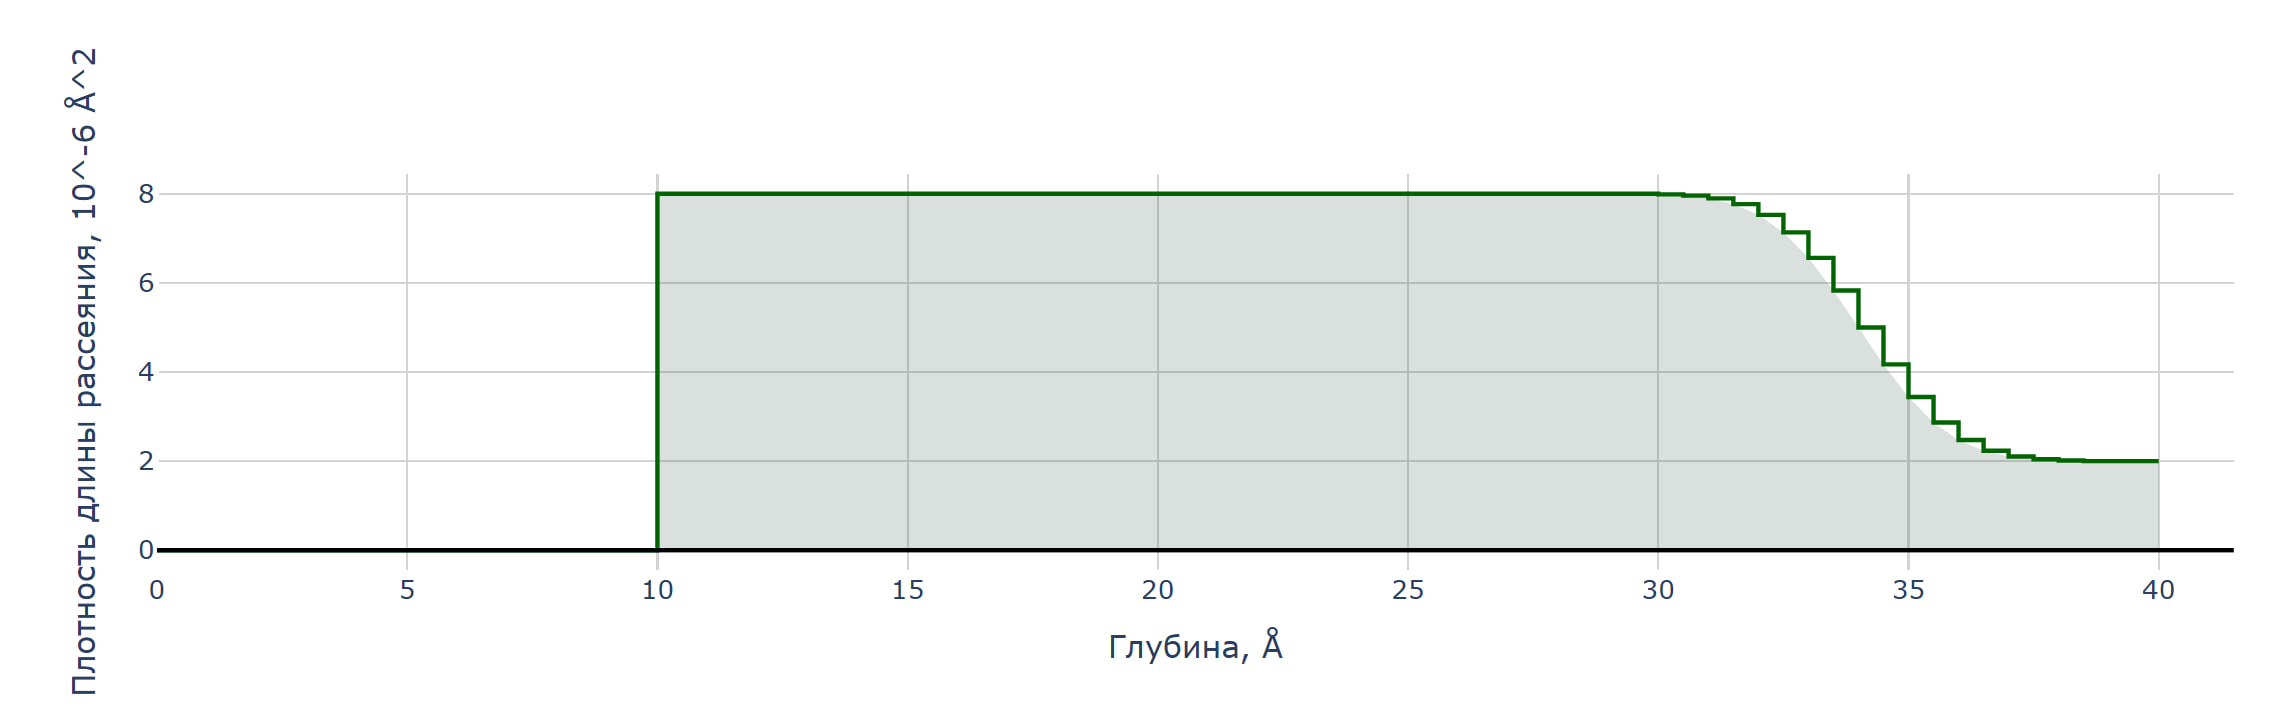
\includegraphics[scale=0.4]{roughness.jpg}
\caption{Модифицированный профиль плотностей длин рассеяния с учётом шероховатости}
\end{figure}

\item \textbf{Динамическая сетка} 

Так как после построения теоретической кривой рефлектометрии к ней будет применена свёртка, необходимо, чтобы для нее было достаточное разрешение: для каждой точки кривой требуется наличие в диапазоне, в котором будет производиться свёртка, того количества точек, которым аппроксимируется гауссов профиль.
С другой стороны, поскольку прямая задача рефлектометрии в последующем будет решаться многократно, требуется ускорить вычисления кривой рефлектометрии. Следовательно, было решено брать минимальное количество точек, необходимое для корректной работы свёртки на моделируемой выборке.
Так, исходя из предположения о локальной гладкости кривой рефлектометрии, можно утверждать, что в диапазоне работы свёртки (зачастую, 11 ближайших точек), шаг сетки остается практически неизменным.
\begin{equation}
    Ndots_{norm}dq_i = 6\sigma q_i,
\end{equation}

где \( \mathrm{Ndots}_{\mathrm{norm}} \) - количество точек, которым аппроксимируется гауссов профиль, 
\( dq_i \) - i-й шаг сетки, 
\( \sigma \) - разрешение установки, 
\( q_i \) - длина волнового вектора на i-й итерации.

Следовательно, получаем рекуррентное соотношение для значений сетки:
\begin{equation}
    q_{i+1} = q_{i} + \frac{6\sigma q_i}{Ndots_{norm}}
\end{equation}

Таким образом, получается минимальный набор точек, необходимый для работы свёртки над моделируемой выборкой измерений.

\subsection{Решение обратной задачи}
Основная сложность в задаче рефлектометрии - это решение обратной задачи рассеяния, поскольку она не имеет решения в общем виде.\\
Необходимо подобрать параметры образца так, чтобы данная (экспериментальная) и моделируемая кривые рефлектометрии совпали, или хотя бы были максимально близки друг к другу.
\item \textbf{Функция ошибок}\\
Для оценки "близости" двух кривых была написана функция, называемая функцией ошибок - чем больше несоответствие, тем больше функция ошибок.\\
В стандартных подходах предлагается использовать критерий Пирсона или среднеквадратическое отклонение по каждой точке кривой рефлектометрии. Критерий Пирсона не подходит уже потому, что вес относительного отклонения будет пропорционален значению коэффициента отражения: 
\begin{equation}
    \chi^2 =\sum{\frac{(\Delta R_i)^2}{R_i}}= \sum{R_i(\frac{\Delta R_i}{R_i})^2}
\end{equation}
Среднеквадратическое отклонение по каждой точке кривой рефлектометрии не имеет такой проблемы, однако, обладает другими свойствами, усложняющими решение задачи.\\
При решении задачи рефлектометрии известны параметры образца: плотности длин рассеяния (задаются материалами образца), глубины слоев материалов. Требуется лишь уточнить глубины слоев с учётом шероховатостей. Так, при поиске в реальных диапазонах параметров, кривая рефлектометрии варьируется не сильно. 
Кроме того, график рефлектометрии из себя представляет сложные затухающие колебания, а информацию об их характере несут минимумы и максимумы, то есть экстремумы. Таким образом, точки на кривой рефлектометрии имеют совершенно разную информативность. Так, например, если "колебания" на двух похожих кривых рефлектометрии будут в "противофазе", но с одинаковым характером "колебаний", то функция ошибок будет велика, несмотря на близость параметров к искомым.\\
Так, функция ошибок среднеквадратическое отклонение по каждой точке имеет не только большое количество локальных минимумов, что существенно осложняет поиск минимума, но и весьма трудоёмка с точки зрения счёта - учитываются все точки кривой рефлектометрии.\\
Ввиду вышеперечисленных факторов, было решено написать свою функцию ошибок, наиболее подходящую для задачи рефлектометрии. Так, функция учитывает только информативные точки с одинаковым весом, относительное отклонение для каждой из них не только по оси ординат, но и по оси абсцисс. 
\begin{figure}[H]
\centering
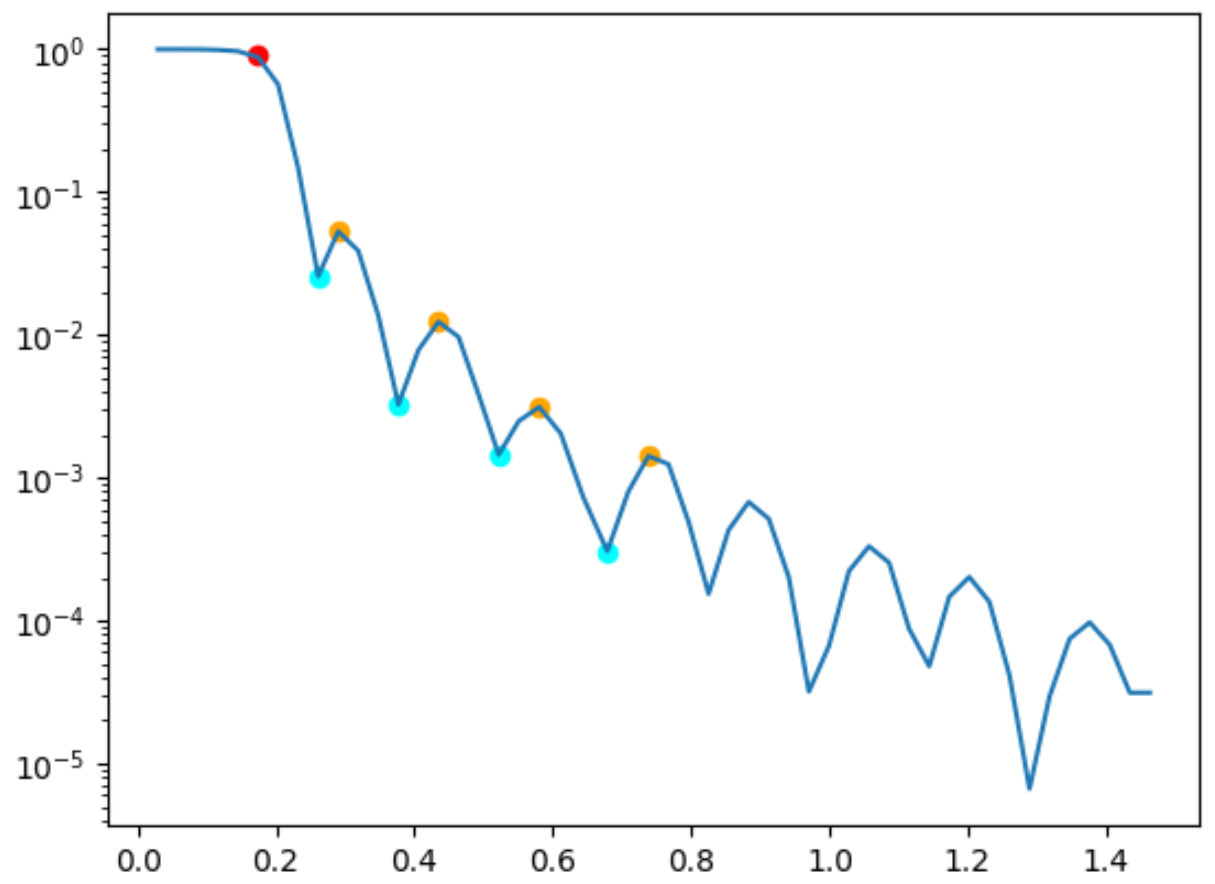
\includegraphics[scale=0.8]{ref_trace.jpg}
\caption{Информативные точки кривой рефлектометрии:\\
критическая точка - красная,\\
первые 4 минимума - голубые,\\
первые 4 максимума - оранжевые.}
\end{figure}


\item \textbf{Поиск минимума функции ошибок} \\
Вышеописанная функция не является строго гладкой и может иметь несколько локальных минимумов, следовательно, наиболее надёжно будут работать стохастические алгоритмы поиска минимума. Однако, такие методы крайне медлительны уже на малых размерностях, а минимум должен быть найден в разумный промежуток времени вне зависимости от числа уточняемых параметров.\\
Следовательно, ввиду относительной гладкости вышеописанной функции, был выбран модифицированный для работы в многомерном кубе алгоритм Бройдена — Флетчера — Гольдфарба — Шанно (L-BFGS-B). Это квазиградиентный метод, что позволяет ему сходиться кратно быстрее, чем стохастическим методам. Градиенты считаются путём численного дифференцирования. 



\end{enumerate}

\subsubsection{Полученные данные}

\textbf{Зависимость коэффициента отражения $R(q_z)$} (рис. 8):

На графике наблюдаются осцилляции, характерные для интерференции нейтронных волн в тонких слоях. Период осцилляций соответствует толщине пленки. После свёртки с аппаратной функцией теоретическая кривая демонстрирует сглаживание осцилляций, имитируя влияние ограниченного разрешения установки.

\begin{figure}[H]
\centering
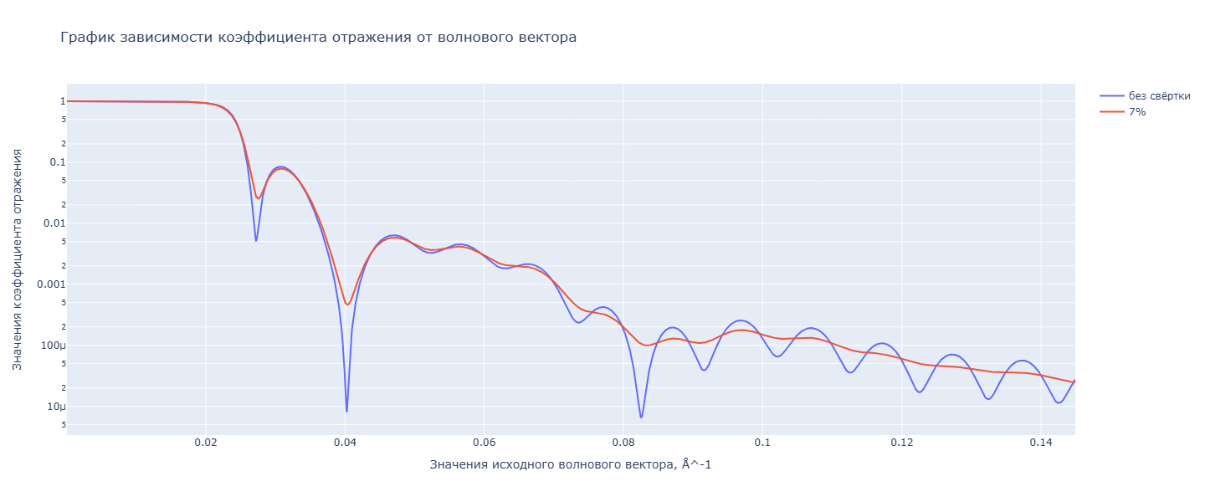
\includegraphics[width=0.9\textwidth]{a0000-img002.png}
\caption{График зависимости коэффициента отражения от волнового вектора}
\end{figure}


\subsection{Выводы по разделу}

Исключение спиновой поляризации упростило модель, сохранив её применимость для немагнитных систем. Векторизация матричных операций повысила эффективность вычислений, что особенно важно для анализа многослойных структур. Модель демонстрирует хорошее согласие с экспериментом, подтверждая её работоспособность для задач рефлектометрии на установках с умеренным разрешением.

\begin{thebibliography}{9}
\bibitem{1} Storn R., Price K. Differential Evolution – A Simple and Efficient Heuristic for Global Optimization over Continuous Spaces. Journal of Global Optimization, 1997. \url{https://web.archive.org/web/20100106073218/http://sci2s.ugr.es/docencia/bioinformatica/bio/ficheros/Apoyo/Tema\%2010/01\%20-\%20DE-Storn-Price-1997.pdf}.
\bibitem{2} Еремеев А.В. Алгоритм дифференциальной эволюции для оптимизации. \url{https://msm.omsu.ru/jrns/jrn63/eremeev.pdf}.
\bibitem{3} Алгоритм дифференциальной эволюции для решения задач многокритериальной безусловной оптимизации. \url{https://cyberleninka.ru/article/n/algoritm-differentsialnoy-evolyutsii-dlya-resheniya-zadach-mnogokriterialnoy-bezuslovnoy-optimizatsii}.
\bibitem{4} Шведов А.С. О методах Монте-Карло с цепями Маркова \url{https://cyberleninka.ru/article/n/o-metodah-monte-karlo-s-tsepyami-markova/viewer}
\bibitem{5} Jonathan Goodman and Jonathan Weare. Ensamble samplers with affine invariance \url{https://msp.org/camcos/2010/5-1/p04.xhtml}

\bibitem{6} Ковальчук М. В., Ильгисонис В. И., Штромбах Я. И., Курский, А. С., Андреев Д. В. Развитие реакторной экспериментальной базы НИЦ «Курчатовский институт»: от пуска Ф-1 до 60-летия реактора ИР-8 \url{https://nrcki.ru/files/pdf/20180301.pdf}

\bibitem{7} Сыромятников В.Г., Ульянов В.А. НЕЙТРОННАЯ РЕФЛЕКТОМЕТРИЯ В РОССИИ: ТЕКУЩЕЕ СОСТОЯНИЕ И ПЕРСПЕКТИВЫ \url{https://www.researchgate.net/publication/357499178_Nejtronnaa_reflektometria_v_Rossii_tekusee_sostoanie_i_perspektivy}

\bibitem{8} А.П. Петраков. Метод рентгеновской рефлектометрии и его применение для исследования лазерного испарения окисной пленки 
с поверхности кремния \url{https://journals.ioffe.ru/articles/viewPDF/7957}

\bibitem{9} S.J.Blundell, J.A.C. Bland. Polarized neutron reflection as a probe of magnetic films ans multilayers \url{https://journals.aps.org/prb/abstract/10.1103/PhysRevB.46.3391}

\bibitem{10} R.N.Watts,D.L.Ederer,R.D.Deslattesand T.B.Lucatorto. Upgraded Facility for Multilayer Mirror Characterization at NIST
\url{https://www.spiedigitallibrary.org/conference-proceedings-of-spie/1547/1/Upgraded-facility-for-multilayer-mirror-characterization-at-NIST/10.1117/12.51284.full}

\bibitem{11} M.Krumrey, M.KUhne, P.MUllerand, F.Schoize. Precisionsoftx-rayreflectometryofcurvedmultilayeroptics \url{https://www.spiedigitallibrary.org/conference-proceedings-of-spie/1547/0000/Precision-soft-x-ray-reflectometry-of-curved-multilayer-optics/10.1117/12.51276.full}

\bibitem{12} Daniel Foreman-Mackey, David W.Hogg, Dustin Lang, Jonathan Goodman. emcee: The MCMC Hammer \url{https://iopscience.iop.org/article/10.1086/670067}

\bibitem{13} В. К. Игнатович. ОДНОМЕРНЫЙ ПЕРИОДИЧЕСКИЙ ПОТЕНЦИАЛ В КВАНТОВОЙ МЕХАНИКЕ. \url{https://journals.nsu.ru/files/sjp/2008/2/0125_Vestnik_NSU_2008T3V2_p99_p107.pdf}

\bibitem{14} Е.О.Серовa, П.С.Савченковa, А.В.Рогачевa, А.И.Калюкановa, В.И.Боднарчукa, А.В.Белушкин. ЭКСПЕРИМЕНТАЛЬНЫЙ СТЕНД ДЛЯ МЕТОДИЧЕСКИХ РАБОТ С ПОЛЯРИЗОВАННЫМИ НЕЙТРОНАМИ НА РЕАКТОРЕ ИР-8 \url{https://journals.eco-vector.com/1028-0960/article/view/686101/ru_RU}

\bibitem{15} Н.К. Плешанов. Нейтронные рефлектометры:
особенности оптимизации, новые перспективы \url{https://oiks.pnpi.spb.ru/media/muromets2015_reports/23-09-15_%D0%9F%D1%80%D0%B5%D0%B4%D0%B8%D1%81%D0%BB%D0%BE%D0%B2%D0%B8%D0%B5/16%2000%20%D0%9F%D0%BB%D0%B5%D1%88%D0%B0%D0%BD%D0%BE%D0%B2%20%D0%9D%D0%9A/PleshanovNK_MURomets-2015.pdf}  

\end{thebibliography}


\end{document}